%% ------------------------------------------------------------
%% TITLE:     Signal and Control - Control - Notes
%% AUTHOR:    BINGHUAN W LI (Dept. Chemical Eng/Bio Eng, Imperial)
%% COMPILED:  XeLaTeX with TeX Live version 2023
%% LICENSE:   This work is licensed under a Creative Commons Attribution-NonCommercial 4.0 International License.
%% ------------------------------------------------------------

% Version History:
% v1.0  - 2021-03 - Initial draft
% v1.1  - 2021-03 - Corrected typos
% v1.2  - 2022-08 - Added diagrams and additional explanations

\documentclass[12pt,a4paper]{article}
\usepackage[margin=2.2cm]{geometry}

\usepackage{fontspec}
    \setmainfont{Times New Roman}
\usepackage{newtxmath}
 
\usepackage{tikzducks}

\usepackage{hyperref}
\hypersetup{hidelinks,
            pdfauthor={Li, Binghuan},
            pdftitle={Signals and Control - Control},
            }


\usepackage{wrapfig}
\usepackage{graphicx, float, subfigure}
\usepackage{fancyhdr}
\usepackage{xcolor}

\usepackage{amsmath, amsfonts, amssymb, mathrsfs, mathtools, cancel}

\usepackage[font={small,it}]{caption}
    \captionsetup[figure]{labelfont={sc},name={Fig.}}

\usepackage{tcolorbox}
    \tcbuselibrary{breakable}

\usepackage[european]{circuitikz}
\usepackage{tikz}
    \usetikzlibrary{shapes,arrows}
    \usetikzlibrary{positioning}
    \usetikzlibrary{calc,patterns,decorations.pathmorphing,decorations.markings}
    \usetikzlibrary{circuits.ee.IEC}
    \tikzstyle{block} = [draw, rectangle, 
    minimum height=1.5em, minimum width=3.5em]
    \tikzstyle{sum} = [draw, circle, node distance=1cm]
    \tikzstyle{input} = [coordinate]
    \tikzstyle{output} = [coordinate]
    \tikzstyle{pinstyle} = [pin edge={to-,thin,black}]


\usepackage{tabularx, booktabs}
\usepackage{sidecap}


    
\usepackage{pgfplots}

\newtcolorbox[auto counter, number within=section]{ex}[2][]{
    breakable, title=Example~\thetcbcounter \ #2, #1}

\newtcolorbox[auto counter, number within=section]{dv}[2][]{
    breakable, title=Derivation~\thetcbcounter: #2, #1}
    
    \setlength{\parindent}{0pt} 
%----------Footer & Header----------%
\pagestyle{fancy}
\fancyhf{}
\lhead{\textit{\leftmark}}
\lfoot{\textbf{\thepage}}%LEFT foot page number

%----------Define \doublerule command----------%
\newcommand{\doublerule}[1][.4pt]{% <===================================
  \noindent
  \makebox[0pt][l]{\rule[.7ex]{0.8\linewidth}{#1}}%
  \rule[0.4pt]{0.8\linewidth}{#1}\par} % <============
  
%----------BEGIN----------%
\begin{document}

%----------Title page----------%
\begin{titlepage}
\centering 
{\Huge Signals and \textit{\underline{Control}}}
\vfill
Last Update: \today
\vspace{1cm}
\hrule
\vspace{1cm}
\textit{This work is licensed under a Creative Commons Attribution 4.0 International License.}
\end{titlepage}

%----------DO NOT CHANGE THE SETTINGS ABOVE----------%
\newpage
% \section*{Acknowledgement}
% I would like to express my deepest appreciation to \emph{Dr. Reiko Tanaka} for her generous help in reviewing these notes with the highest profession.
% \ \\ \\
% I would like to extent my sincere thanks to \emph{Ashira Meyer}, \emph{Aron Lajko}, \emph{Daniel Duffill}, \emph{Kenny Panteleev}, \emph{Peter Xie}, \emph{Weixun Luo} and \emph{rep group} for their insightful comments and suggestions that have continuously improved this note. Their work significantly optimized the structure. 
% \ \\ \\
% Special thanks to \emph{Haroon Chughtai}. His notes greatly enlightened me when preparing this new set.

\newpage
\tableofcontents
\newpage

%-------------------------------------------%
\section{Laplace Transform}
%-------------------------------------------%
\textbf{Fourier Transform:}
\[ 
    F(\omega) = \mathcal{F} (f(t)) = \int_{-\infty}^{+\infty} f(t) e^{-j\omega t} \mathrm{d}t 
\]
\textbf{Laplace Transform:}
\[ 
    F(s) = \mathcal{L} (f(t)) = \int_{-\infty}^{+\infty} f(t) e^{-st} \mathrm{d}t 
\]
\quad where $s = \sigma + j \omega$.
\ \\
\begin{itemize}
    \item \textbf{Reason we need Laplace transform:}
    \begin{itemize}
        \item  Laplace transform is the generalization of Fourier transform. It is defined for a larger class of functions than Fourier transform.
        \item This is because $s$ can be defined anywhere in the complex plane.
    \end{itemize}
    
    \item In control, we usually take the lower boundary of the integral to 0, rather than $-\infty$. We call this \textbf{unilateral Laplace transform}. \[ F(s) = \mathcal{L} (f(t)) = \int_{0}^{\infty} f(t) e^{-st} \mathrm{d}t \]
%---------------EXAMPLE START---------------%
    \begin{ex}{}
     Fourier transform does not exist for $f(t)=e^{t}$, this is because $f(t)$ is not convergent.\\\\
     However, we can find the Laplace transform of  $f(t)=e^{t}$. \[ F(s) = \mathcal{L} (e^{t}) = F(s) = \mathcal{L} (f(t)) = \int_{0}^{\infty} e^{(1-s)t}  \mathrm{d}t  = -\frac{1}{1-s} \] This provided that \[ \lim_{t \to \infty} e^{(1-s)t} = 0 \] which is true for $s$ such that $\Re(s)>1$.
    \end{ex}
%---------------EXAMPLE END---------------%
    \item We make the signal \textbf{converge} ($e^{-\sigma t} \cdot f(t)$ converges) by multiplying $e^{-\sigma t}$, so that it can be analysable.
    \[
    e^{-st} = e^{-(\sigma + j\omega)t} = e^{-\sigma t}\cdot e^{-j\omega t} 
    \]
\end{itemize}

%-------------------------------------------%
\subsection{Table of Laplace Transform} 
%-------------------------------------------%
\begin{table}[H]
    \centering
    \caption{Table of Laplace transform}
    \begin{tabular}{p{3cm} p{3cm} p{3cm}}
        \toprule
        & $\boldsymbol{f(t)}$ & $\boldsymbol{F(s)}$\\ 
        \midrule
        Time delay  &       $ \delta(t-\tau)$ &     $\displaystyle e^{-\tau s}$ \\ [2ex] 
        Impulse     &       $\delta(t)$  &          $1$ \\ [2ex] 
        Step        &       $u(t)$ &                $\displaystyle \frac{1}{s}$  \\  [2ex] 
        Ramp        &       $t$ &                   $\displaystyle \frac{1}{s^{2}}$  \\ [2ex] 
        Exponential &       $e^{-at}$ &             $\displaystyle \frac{1}{s+a}$  \\ [2ex] 
        Sine        &       $\sin(\omega_{0} t)$ &  $\displaystyle \frac{\omega}{s^{2}+\omega_{0}^{2}}$\\ [2ex]
        Cosine      &       $\cos(\omega_{0} t)$ &  $\displaystyle \frac{s}{s^{2}+\omega_{0}^{2}}$ \\ [1.6ex]
        \bottomrule
    \end{tabular}
\end{table}

\begin{dv}{Time delay}
Let $g(t)=f(t-T)$, take Laplace transform
\begin{align*}
\begin{split}
    G(s) &= \int_{0}^{+\infty}e^{-st}g(t)\mathrm{d}t =  \int_{0}^{+\infty}e^{-st}f(t-T)\mathrm{d}t\\
    &= \int_{0}^{+\infty}e^{-s(\tau+T)}f(\tau)\mathrm{d}\tau = e^{-sT}\underbrace{\int_{0}^{+\infty}e^{-s\tau}f(\tau)\mathrm{d}\tau}_{F(s)} \\
    &= e^{-sT}F(s)
\end{split}
\end{align*}
\end{dv}
%---------------EXAMPLE START---------------%
\begin{ex}{}
Evaluate $\mathcal{L}[\sin(2t-3)]$.
\vspace{.3cm} \hrule \vspace{.3cm} 
Let $f(t) = \sin(2t)$, take Laplace transform: $\displaystyle F(s) = \frac{2}{s^{2}+4}$.\\\\
Due to $\delta(t-\tau)  \xrightarrow{\mathcal{L}} e^{-\tau s}$
\[\mathcal{L}[\sin(2t-3)] = \mathcal{L}[\sin2(t-\frac{3}{2})] = e^{-\frac{3}{2}s}\frac{2}{s^{2}+4}\]
\end{ex}
%---------------EXAMPLE END---------------%

%-------------------------------------------%
\subsection{Properties of Laplace Transform}
%-------------------------------------------%
\begin{table}[H]\centering
    \caption{Properties of Laplace transform}
    \begin{tabular}{p{4cm} p{3cm} p{6cm}}
    \toprule
    & $\boldsymbol{f(t)}$ & $\boldsymbol{F(s)}$\\ \midrule
    Linearity & $af(t)+bg(t)$ & $aF(s)+bG(s)$ \\ [1.5ex] 
    
    Differentiation & $f'(t)$  & $ sF(s)-f(0)$ \\
    &&$s^{n}F(s)-s^{n-1}f(0)-...-  f^{n-1}(0)$\\[1.5ex] 
    
    Integration& $\int_{0}^{t}f(\tau)\mathrm{d}\tau$ &  $\displaystyle \frac{1}{s} F(s)$  \\  [1.5ex] 
    Convolution&  $f(t)*g(t)$ & $F(s)G(s)$  \\ [1.5ex]
    
    Exponential scaling & $e^{-at}f(t)$ & $F(s+a)$  \\ [1.5ex] 
    
    Time scaling & $f(at)$ & $\displaystyle \frac{1}{a}F(\frac{s}{a})$\\ [1.5ex] 
    
    Time shifting & $f(t-\tau)u(t-\tau)$ & $e^{-\tau s}F(s)$ \\ [1.5ex] 
    \bottomrule
\end{tabular}
\end{table}

\begin{dv}{Exponential scaling}
Let $g(t)=e^{-at}f(t)$, take Laplace transform:
\begin{align*} 
    \begin{split}
        G(s) &= \int_{0}^{\infty}e^{-st}g(t) \mathrm{d}t\\
        &=\int_{0}^{\infty}e^{-st}e^{-at}f(t) \mathrm{d}t\\
        &= \int_{0}^{\infty}e^{-(s+a)t}f(t) \mathrm{d}t\\
        &= F(s+a)
    \end{split} 
\end{align*}
\end{dv}
%---------------EXAMPLE START---------------%
\begin{ex}{}
Evaluate $ \mathcal{L}[e^{-t}\sin(2t)]$.
\vspace{.3cm} \hrule \vspace{.3cm} 
Let $f(t) = \sin(2t)$, take Laplace transform: $\displaystyle F(s) = \frac{2}{s^{2}+4}$.\\\\
Due to $e^{-at}f(t) \ \xrightarrow{\mathcal{L}}  \ F(s+a)$
\[\mathcal{L}[e^{-t}\sin(2t)] = F(s+1) = \frac{2}{(s+1)^{2}+4}\]
\end{ex}
%---------------EXAMPLE END---------------%

%-------------------------------------------%
\section{ODE description of LTI systems}
%-------------------------------------------%
    \begin{figure}[H] 
        \centering
        % 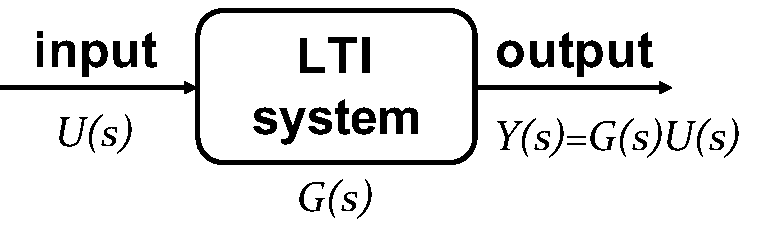
\includegraphics[width=0.4\textwidth]{images/LTI_independent.pdf}
        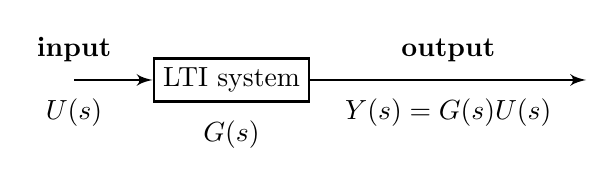
\begin{tikzpicture}[auto, node distance=2cm,>=latex',line width=1pt]
\centering
    \node [input, name = input] {};
    \node [block, right of = input] (controller) {LTI system};
    \node [output, right= 3.5cm of controller] (output) {};

    \draw [draw,->] node[below=.1cm] {$U(s)$} node[above=.1cm] {\textbf{input}}(input) --  (controller) node [below=.1cm of controller]{$G(s)$};
    \draw [->] (controller) -- node[below=.1cm] {$Y(s)= G(s)U(s)$} node[above=.1cm] {\textbf{output}} (output);
\end{tikzpicture}
        \caption{Linear time-invariant system}
    \end{figure}
    
\begin{itemize}
    \item LTI systems can be described by ODEs with constant coefficients in time domain:
        \[ a_{n} \frac{d^{n}y(t)}{dt^{n}}+...+a_{1} \frac{dy(t)}{dt}+a_{0} y(t) = b_{m} \frac{d^{m}u(t)}{dt^{m}}+...+b_{1} \frac{du(t)}{dt}+b_{0} u(t) \]

    \item Assuming there is zero initial conditions, take Laplace transform:
        \[ a_{n} s^{n} Y(s)+...+ a_{1} s Y(s) + a_{0} Y(s) = b_{m} s^{m} U(s)+...+b_{1} s U(s) + b_{0} U(s) \]
        \ where $\mathcal{L}[y(t)] = Y(s)$ and $\mathcal{L}[u(t)] = U(s)$. 

    \item \textbf{Transfer Function} is defined as:
        \[ \boxed{G(s)=\frac{Y(s)}{U(s)}=\frac{b_{m} s^{m}+...+b_{1} s +b_{0}}{a_{n} s^{n}+...+a_{1} s+a_{0}},\quad m \leq n }\] 
        
        \begin{itemize}
             \item Laplace transform of \textbf{output} divided by Laplace transform of \textbf{input}, assuming zero initial conditions.
             
             \item Ratio of polynomial in $s$.
             
             \item Transfer function is independent of the form of the input
        \end{itemize}
\end{itemize}
\ \\
\textbf{Properties of transfer functions:}
\begin{itemize}
    \item Linear functions
        \[ 
        G(s) (aU_{1}(s)+bU_{2}(s)) = aG(s)U_{1}(s)+b G(s) U_{2}(s)
        \]
    \item Commutative
        \[G_{1}(s) G_{2}(s) = G_{2}(s)G_{1}(s)\]
    \item Associative
        \[G_{1}(s) +G_{2}(s) = G_{2}(s) +G_{1}(s)\]
\end{itemize}

%---------------EXAMPLE START---------------%
\begin{ex}{Mass-Spring-Damper system}
    \begin{figure}[H] 
        \centering
        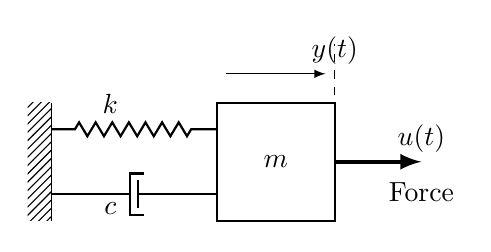
\begin{tikzpicture}[every node/.style={draw,outer sep=0pt,thick}]
    \tikzstyle{spring}=[thick,decorate,decoration={zigzag,pre length=0.3cm,post length=0.3cm,segment length=6}]
    \tikzstyle{damper}=[thick,decoration={markings,  
      mark connection node=dmp,
      mark=at position 0.5 with 
      {
        \node (dmp) [thick,inner sep=0pt,transform shape,rotate=-90,minimum width=15pt,minimum height=3pt,draw=none] {};
        \draw [thick] ($(dmp.north east)+(2pt,0)$) -- (dmp.south east) -- (dmp.south west) -- ($(dmp.north west)+(2pt,0)$);
        \draw [thick] ($(dmp.north)+(0,-5pt)$) -- ($(dmp.north)+(0,5pt)$) ; 
      }
    }, decorate]
    \tikzstyle{ground}=[fill,pattern=north east lines,draw=none,minimum width=0.75cm,minimum height=0.3cm]
    
    \node (M) [minimum width=1.5cm, minimum height=1.5cm] {$m$};
    \node (arrowstart) [name=arrowstart, above = 1cm of M.west,draw=none]{};
    \node (arrowend) [name=arrowend, above= 1cm of M.east,draw=none]{};
    
    \node (wall) [ground, rotate=-90, minimum width=1.5cm,yshift=-3cm] {};
    \draw (wall.north east) -- (wall.north west);
    
    % no need for ground, commented out
    % \node (gnd) [ground, rotate=0, minimum width=5cm,yshift=-0.9cm, xshift=-0.65cm] {};
    % \draw (wall.south east) -- (M.south east)--+(1.1cm,0);
    
    \draw [spring] (wall.160) -- ($(M.north west)!(wall.160)!(M.south west)$);
    \draw [damper] (wall.20) -- ($(M.north west)!(wall.20)!(M.south west)$);
    
    \draw [-latex,ultra thick] (M.east) ++ (0,0) -- +(1.1cm,0) node [above, draw=none]{$u(t)$} node [below=.15cm,draw=none]{Force};
    \draw [dashed] (M.east) ++ (0,0) -- +(0,1.5cm);
    \draw [-latex] (arrowstart) -- (arrowend) node[draw=none, above]{$y(t)$};
    
    \node[below=.3cm, draw=none] at (-2.1,-0.1){$c$};
    \node[above, draw=none] at (-2.1,0.5){$k$};
\end{tikzpicture}
    \end{figure}
    A Mass-Spring-Damper system can be characterized by ODE:
    \[ m\frac{d^{2}y(t)}{dt^{2}}+c\frac{dy(t)}{dt}+ky(t)=u(t) \]
    Take Laplace transform with zero initial condition:
    \[ ms^{2}Y(s)+csY(s)+kY(s)=(ms^{2}+cs+k)Y(s)=U(s) \]
    So the transfer function is 
    \[ G(s)=\frac{Y(s)}{U(s)}= \frac{1}{ms^{2}+cs+k} \]
    If m=6, c=5 and k=1, 
    \begin{itemize}
    \item to find the impulse response:
    \[ 
    Y(s) = G(s)U(s) = G(s) 
    = \frac{1}{6s^{2}+5s+1} 
    = \frac{-2}{2s+1}+\frac{3}{3s+1}= \frac{-1}{s+0.5}+\frac{1}{s+\frac{1}{3}} 
    \]
    \[ 
    y(t) = g(t) 
    = \mathcal{L}^{-1} [G(s)] 
    = -e^{-t/2}+-e^{-t/3} 
    \]
    
    \item to find the step response:
    \[
    Y(s) = G(s)U(s) = \frac{1}{s}\frac{1}{6s^{2}+5s+1} 
    = \frac{4}{2s+1}-\frac{9}{3s+1} +\frac{1}{s} 
    = \frac{2}{s+\frac{1}{2}}-\frac{3}{s+\frac{1}{3}} +\frac{1}{s} \]
    \[ y(t) = 2e^{-t/2}-3^{-t/3} +1 \]
    \end{itemize}
    
    \textbf{Comments:}
    \begin{itemize}
     \item From the example above, the solutions of denominator of the transfer function are $s = -\frac{1}{2}$ and $s = -\frac{1}{3}$;
     
     \item These two solutions are the \textbf{poles} of the system. 
     \item Poles define the long-time behaviours of the system: whether the system can stay at certain level, or converges to 0 or $\infty$.
     
     \item $s = -\frac{1}{2}$ and $s = -\frac{1}{3}$ are real, negative solutions, so as $t\to \infty$, 
     for step response,  $y(t) \to 1$, (and for impulse response, $y(t) \to 0$). They have no affect on long-term behaviour of the system.
    \end{itemize}
\end{ex}
%---------------EXAMPLE END---------------%

%-------------------------------------------%
\subsection{Zero-pole-gain}
%-------------------------------------------%
Transfer function can be written as:
\begin{align*}
\begin{split}
    G(s)
    &=\frac{Y(s)}{U(s)}=\frac{b_{m} s^{m}+...+b_{1} s +b_{0}}{a_{n} s^{n}+...+a_{1} s+a_{0}}\\
    &=\boxed{K\frac{(s-z_{1})(s-z_{2})...(s-z_{m})}{(s-p_{1})(s-p_{2})...(s-p_{n})}}\\
\end{split}
\end{align*}
\ where $K$ is the gain.

 \begin{itemize}
      \item Zeros $\{z_{1} , \ z_{2}, \ ..., \ z_{m}\}$ are the solutions of $N(s)=0$;
      \item Poles $\{p_{1} , \ p_{2}, \ ..., \ p_{n}\}$ are the solutions of $D(s)=0$;
 \end{itemize}

%---------------EXAMPLE START---------------%
\begin{ex}{}
Find the poles and zeros of a LTI system
    \[\frac{d^{2}y}{dx^{2}}+5\frac{dy}{dx}+6y = 2\frac{du}{dt}+u\]
\hrule
\vspace{.3cm}
\begin{enumerate}
    \item Obtain the transfer function by Laplace transform
        \[s^{2}Y(s)+5sY(s)+6Y(s) = 2sU(s)+U(s)\]
        This gives
        \[G(s) =\frac{Y(s)}{U(s)} = \frac{2s+1}{s^{2}+5s+6}\]
        
    \item Factorize the transfer function
        \begin{itemize}
            \item $2s+1=0$, zero at $s = -\frac{1}{2}$.
            \item $(s+3)(s+2)=0$, poles at $s = -2$ and $s = -3$
        \end{itemize}
\end{enumerate}
\end{ex}
%----------------EXAMPLE END----------------%
%---------------EXAMPLE START---------------%
\begin{ex}{}
Find the ODE representing the system with 
\begin{itemize}
    \item poles at $-1\pm 2j$
    \item zero at -4 
    \item gain factor 3
\end{itemize}
\hrule
\vspace{.3cm}
\begin{enumerate}
    \item Find the transfer function:
    \[
    G(s) = \frac{Y(s)}{U(s)} 
    = 3\frac{s-(-4)}{[s-(-1-2j)][s-(-1+2j)]} 
    = 3\frac{s+4}{s^{2}+2s+5}
    \]
    
    \item ODE can be found by taking Inverse Laplace transform:
    \[
    (s^{2}+2s+5)Y(s) = 3(s+4)U(s)
    \quad \xrightarrow{\mathcal{L}} \quad
    \frac{d^{2}y}{dt^{2}}+2\frac{dy}{dt}+5y 
    = 3\frac{du}{dt}+12u 
    \]
\end{enumerate}
\end{ex}
%----------------EXAMPLE END----------------%


%-------------------------------------------%
\subsection{Block Diagrams}
%-------------------------------------------%
Block diagrams are used to visually represent LTI systems.
\begin{figure}[H] \centering
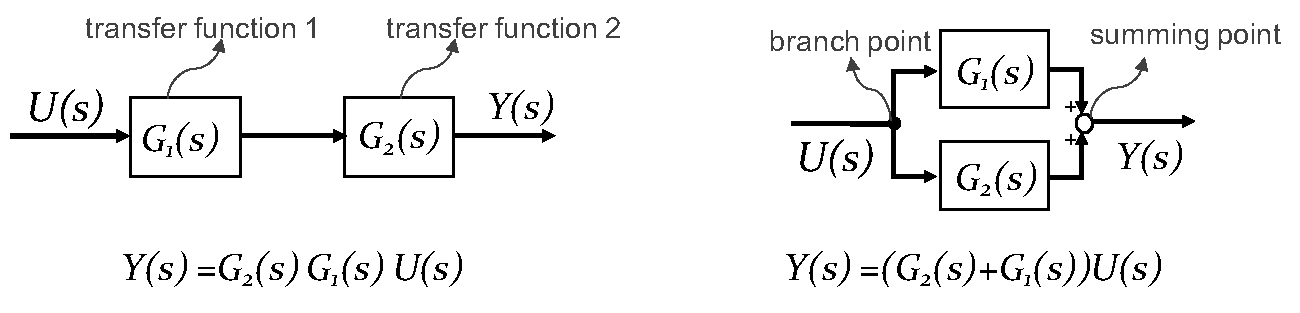
\includegraphics[width=.9\textwidth]{images/block_diagram.pdf}
\caption{Block diagram explanation}
\end{figure}

%---------------EXAMPLE START---------------%
\begin{ex}{}
Consider the simplest negative feedback system, as shown below. Find the transfer function of the system.
\begin{figure}[H] 
    \centering
    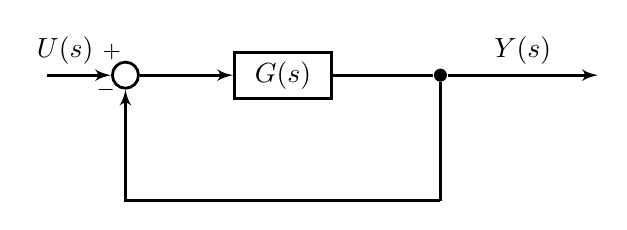
\begin{tikzpicture}[auto, node distance=2cm,>=latex',line width=1pt]
    \node [input, name=input] {};
    \node [sum, right of=input] (sum) {};
    \node [block, right of=sum] (controller) {$G(s)$};
    \coordinate [right of = controller, circle, scale=0.5, fill](tooutput){};
    \node [output, right of=tooutput] (output) {};
    \coordinate [below= 1.5cm of tooutput] (measurements) {};

    \draw [draw,->] (input) -- node {$U(s)$\ {\footnotesize$+$}} (sum); 
    \draw [->] (sum) -- node {} (controller);
    \draw [-] (controller) -- (tooutput);
    \draw [->] (tooutput) -- node[] {$Y(s)$} (output);
    \draw [-] (tooutput) |- (measurements);
    \draw [->] (measurements) -| 
    node[pos=1] {{\footnotesize$-$}} (sum);
\end{tikzpicture}
\end{figure}
\hrule \vspace{.3cm} 
\textit{Note:} \  the minus sign in the figure indicates the negative feedback in the system.
\[ Y(s) = G(s)(U(s)-Y(s))\]
Rearrange, then we find the transfer function of this closed-loop system:
\[\boxed{\frac{Y(s)}{U(s)} = \frac{G(s)}{1+G(s)}}\]
\end{ex}
%----------------EXAMPLE END----------------%
%---------------EXAMPLE START---------------%
\begin{ex}{} 
Derive the transfer function of the following negative feedback system.
\begin{figure}[H] 
    \centering
    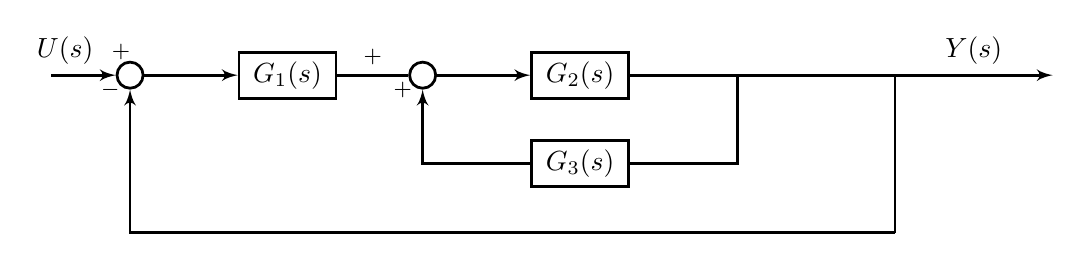
\begin{tikzpicture}[auto, node distance=2cm,>=latex',line width=1pt]
    \node [input, name = input] {};
    \node [sum, right of = input] (sum) {};
    \node [block, right of = sum] (controller1) {$G_{1}(s)$};
    \node [sum, right = 0.9cm of controller1] (sum2) {};
    \node [block, right of= sum2] (controller2) {$G_{2}(s)$};
    \node [block, below= 0.5cm of controller2] (controller3) {$G_{3}(s)$};
    \coordinate [right of = controller2](right2con2){};
    \coordinate [right of = right2con2](tooutput){};
    \node [output, right of = tooutput] (output) {};
    \coordinate [below = 2cm of tooutput] (measurements) {};

    \draw [draw,->] (input) -- node {$U(s)$ \ {\footnotesize$+$}} (sum); 
    \draw [->] (sum) -- node {} (controller1);
    \draw [->] (controller1) -- node {{\footnotesize$+$}} (sum2) -- (controller2);
    \draw [-] (controller2) -- (right2con2) |- (controller3);
    \draw [->] (controller3) -| node[pos=1] {{\footnotesize$+$}}(sum2);
    \draw [-] (controller2) -- (tooutput);
    \draw [->] (tooutput) -- node[] {$Y(s)$} (output);
    \draw [-] (tooutput) |- (measurements);
    \draw [->] (measurements) -| 
    node[pos=1] {{\footnotesize$-$}} (sum);
\end{tikzpicture}
\end{figure}
\hrule \vspace{.3cm} 
Consider the dashed section: 
\begin{figure}[H] 
    \centering
    % 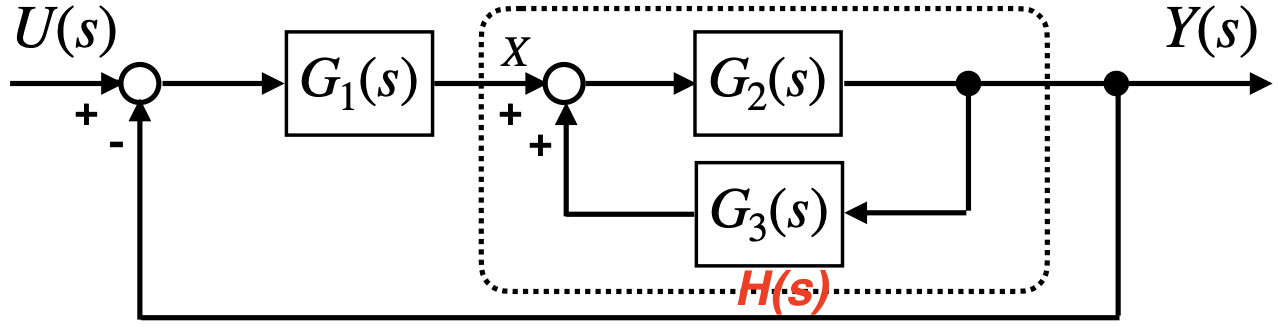
\includegraphics[width=.5\textwidth]{images/BD2_dashed.png}
    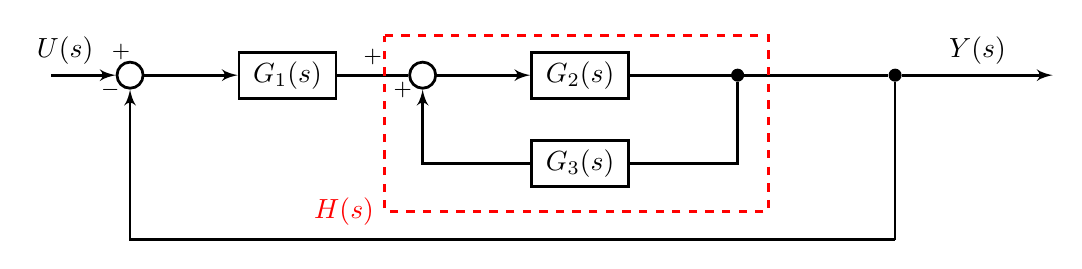
\begin{tikzpicture}[auto, node distance=2cm,>=latex',line width=1pt]
    \node [input, name = input] {};
    \node [sum, right of = input] (sum) {};
    \node [block, right of = sum] (controller1) {$G_{1}(s)$};
    \node [sum, right = 0.9cm of controller1] (sum2) {};
    \node [block, right of= sum2] (controller2) {$G_{2}(s)$};
    \node [block, below= 0.5cm of controller2] (controller3) {$G_{3}(s)$};
    \coordinate [right of = controller2, circle, scale=0.5, fill](right2con2){};
    \coordinate [right of = right2con2, circle, scale=0.5, fill](tooutput){};
    \node [output, right of = tooutput] (output) {};
    \coordinate [below = 2cm of tooutput] (measurements) {};

    \draw [draw,->] (input) -- node {$U(s)$ \ {\footnotesize$+$}} (sum); 
    \draw [->] (sum) -- node {} (controller1);
    \draw [->] (controller1) -- node {{\footnotesize$+$}} (sum2) -- (controller2);
    \draw [-] (controller2) -- (right2con2) |- (controller3);
    \draw [->] (controller3) -| node[pos=1] {{\footnotesize$+$}}(sum2);
    \draw [-] (controller2) -- (tooutput);
    \draw [->] (tooutput) -- node[] {$Y(s)$} (output);
    \draw [-] (tooutput) |- (measurements);
    \draw [->] (measurements) -| 
    node[pos=1] {{\footnotesize$-$}} (sum);
    
    \draw[red, dashed] ([xshift=-3mm, yshift=5mm]sum2.west) -- ([xshift=3mm, yshift=5mm]right2con2.east) |- ([yshift=-3mm]controller3.south) -| node[left]{$H(s)$} ([xshift=-3mm, yshift=5mm]sum2.west);
\end{tikzpicture}
\end{figure}
The transfer function of the dashed section, $H(s)$, that is equivalent to the combination of $G_{2}(s)$ and $G_{3}(s)$.
\begin{itemize}
    \item Let the input to the dashed section be $X(s)$:
        \[Y(s) = G_{2}(s)(X+G_{3}(s)Y(s))\]
    \item Rearrange:
        \[
        H(s) = \frac{Y(s)}{X(s)} = \frac{G_{2}(s)}{1-G_{2}(s)G_{3}(s)}
        \]
\end{itemize}
Then we are going to find the equivalent transfer function to the whole system:
\[Y(s) =(U(s)-Y(s))G_{1}(s)H(s)\]
This gives us the final result:
\[
T.F. \ = \ 
\frac{Y(s)}{U(s)} = 
\frac{G_{1}(s)H(s)}{1+G_{1}(s)H(s)}, \quad \text{where} \ 
H(s) = \frac{G_{2}(s)}{1-G_{2}(s)G_{3}(s)}
\]
\end{ex}
%----------------EXAMPLE END----------------%

%-------------------------------------------%
%-------------------------------------------%
\section{Poles and Stability}
%-------------------------------------------%
Poles are the solutions of the characteristic equation(the denominator of a transfer function) which defines the stability of the system.\\\\
The impulse response have different look when their poles have different locations in the s-domain.
\begin{itemize}
    \item \textbf{Poles at:} $s = \sigma \pm \mathbf{j}\omega$
    
    \item \textbf{Impulse response:}
    \[ g(t) = Ae^{(\sigma \pm \mathbf{j}\omega)t} = Ae^{\sigma t}(\cos(\omega t)\pm\mathbf{j}\sin(\omega t))\]
    \ where $\omega$ is the frequency of the oscillation.
\end{itemize}

\begin{figure}[H] 
    \centering
    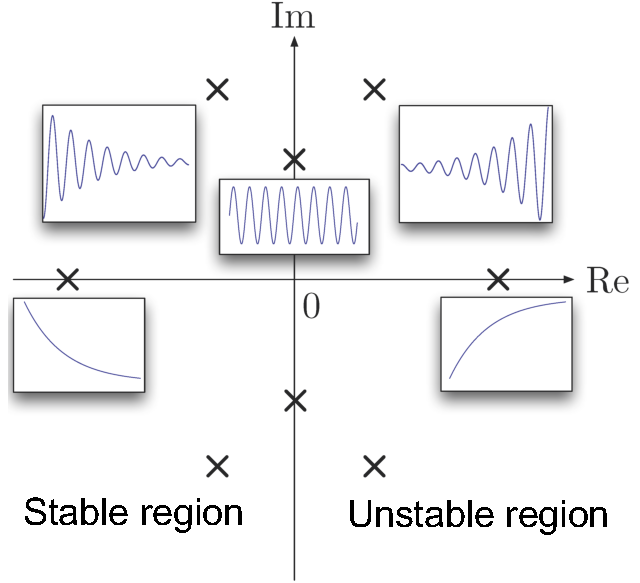
\includegraphics[width=.45\textwidth]{images/pole_location.pdf}
    \caption{Pole location}
\end{figure}

Stability is evaluated by the signs of the real parts of the poles:
\begin{itemize}
    \item \textbf{Asymptotic stability}: when $\Re\{p_{i}\} < 0 $ for all poles $p_{i}$: (\textsc{Fig. 3} - stable region)
        \begin{itemize}
            \item The output decays within an exponential envelope approaching asymptotically 0. 
        \end{itemize}
        
    \item \textbf{Instability} when at least one pole is $\Re\{p_{i}\} >0$: (\textsc{Fig. 3} - unstable region)
        \begin{itemize}
            \item The output grows without bound. 
        \end{itemize}
        
    \item \textbf{Marginal stability} when $\Re\{p_{i}\} =0$ for some poles and $\Re\{p_{i}\} <0$ for all other poles: (\textsc{Fig. 3} - middle)
        \begin{itemize}
            \item The output never decays or grows in amplitude, and shows sustained oscillations. 
        \end{itemize}
\end{itemize}
%-------------------------------------------%
%-------------------------------------------%
\subsection{Finding Stability}
%-------------------------------------------%
We have 2 methods to find the stability of the system:
\begin{enumerate}
    \item \textbf{Solving the characteristic equation} to find poles. The signs of the real part of the poles indicates the stability of the system.
    \item \textbf{Routh stability criterion}. This is particularly useful if the characteristic equation is of high order and tedious to solve.
\end{enumerate}
%*******************************************%

%-------------------------------------------%
\subsubsection{Routh Stability Criterion}
%-------------------------------------------%
Routh Table can determine the number of poles with positive real parts.
\begin{itemize}
\item We only care about the denominator of the transfer function. 
\item Key concept: \textbf{The number of change of sign in the 1st column  = number of poles with positive real parts.}
\end{itemize}
\ \\
\underline{\textbf{To create a Routh Table:}}
\begin{itemize}
\item Given the transfer function:
    \[G(s) = \frac{N(s)}{D(s)}\]
    and 
    \[D(s) = a_{n}s^{n}+a_{n-1}s^{n-1}+\ldots+a_{1}s+a_{0}\]
    
    \item Fill in the corresponding values to the Routh Table:
        \begin{table}[H]
            \centering 
            \begin{tabular}{c|c|c|c}
                 $s^{n}$ & $a^{n}$ & $a^{n-2}$ & $a^{n-4}$\\ \hline
                 $s^{n-1}$ & $a^{n-1}$ & $a^{n-3}$ & $a^{n-5}$\\ \hline \hline
                 $s^{n-2}$ & $b^{(n-2)}_{1}$ & $b^{(n-2)}_{2}$ & $b^{(n-2)}_{3}$ \\ \hline 
                 $s^{n-3}$ & $b^{(n-3)}_{1}$ & $b^{(n-3)}_{2}$ & $b^{(n-3)}_{3}$\\ \hline
                 $\vdots$&$\vdots$&$\vdots$&\\ \hline
                 $s^{2}$ & $b^{(2)}_{1}$ & $b^{(2)}_{2}$ & 0 \\ \hline
                 $s^{1}$ & $b^{(1)}_{1}$ & 0 & \\ \hline
                 $s^{0}$ & $b^{(0)}_{1}$ & &\\ \hline
            \end{tabular}
         \end{table}
         
         \begin{minipage}{.4\textwidth}
         where 
         \[b_{i}^{(k)} = \frac{b_{1}^{(k+1)}\times b_{i+1}^{(k+2)} - b_{1}^{(k+2)}\times b_{i+1}^{(k+1)}}{b_{1}^{(k+1)}}\]
         \end{minipage}\hfill
        \begin{minipage}{.6\textwidth}
            \begin{figure}[H] 
                \centering
                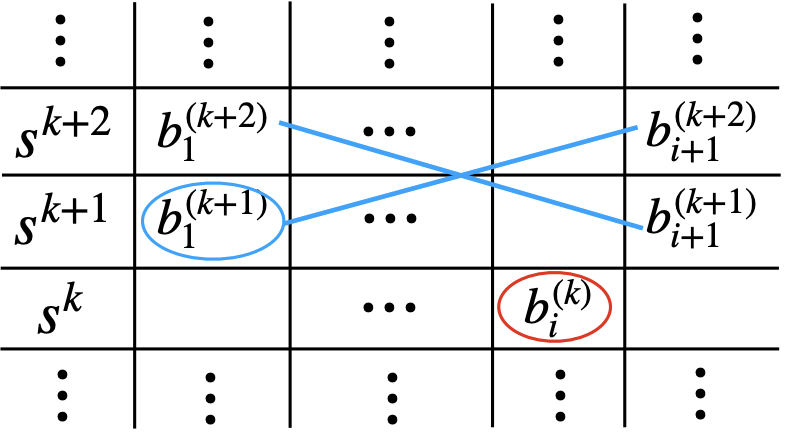
\includegraphics[width=.7\textwidth]{images/routh.png}
            \end{figure}
        \end{minipage}
        
    \item The system is asymptotically stable \textit{if and only if}
        \begin{itemize}
            \item $a_{i}>0 ,\ \forall i$ (for all $i$ values)
            \item \textbf{no change of sign} in the 1st column of the Routh Table.
        \end{itemize}
\end{itemize}
%---------------EXAMPLE---------------%
\begin{ex}{}
Given the transfer function $\displaystyle G(s) = \frac{2s+1}{s^{2}+5s+6}$, evaluate the stability of the system.\\
\begin{minipage}{0.3\textwidth}
     \begin{table}[H]
        \begin{tabular}{c|c|c}
            $s^{2}$&1&6\\ \hline
            $s^{1}$&5&0\\ \hline \hline 
            $s^{0}$&$\frac{6\times 5 -1\times 0}{5}=6$&\\ 
        \end{tabular}
     \end{table}
\end{minipage} \hfill
\begin{minipage}{0.7\textwidth}
 No change of sign in the 1st column since $1\to 5\to 6$. \\ Therefore, it has 0 unstable poles.
 \end{minipage} \ \\ \\
\textit{Note: for the cells with no value from the characteristic function, but this cell is involved in calculation, fill in 0 instead.}
\end{ex}
%----------------EXAMPLE END----------------%
%---------------EXAMPLE START---------------%
\begin{ex}{}
Given the transfer function $\displaystyle G(s) = \frac{2s+1}{s^{3}+s^{2}+3s+10}$, evaluate the poles.\\\\
\begin{minipage}{0.5\textwidth}
    \begin{table}[H]
        \begin{tabular}{c|c|c|c}
            $s^{3}$&1&3&0\\ \hline
            $s^{2}$&1&10&0\\ \hline \hline
            $s^{1}$&$\frac{3\times -1\times 10}{1}=-7$&(\textit{assume}) $x$(=0)& \\ \hline 
            $s^{0}$&$\frac{-7\times 10 -1\times x}{-7}=10$&&\\ 
        \end{tabular}
    \end{table}
 \end{minipage} \hfill
 \begin{minipage}{0.4\textwidth}
    To find the value of $x$:
    \[x = \frac{10\times0-3\times0}{1}=0\]
 \end{minipage}\\\\\\
  It has 2 unstable poles since the sign has changed twice($1\to 1\to -7 \to 10$) in the first column.
  \ \\ \\
 \textit{Note: add a column to the right when necessary.}
\end{ex}
%----------------EXAMPLE END----------------%


%-------------------------------------------%
\subsection{Final Value Theorem}
%-------------------------------------------%
Final value theorem:
\[\lim_{t\to \infty}y(t) = \lim_{s\to 0}sY(s)\]
\ \ where 
\[y(t) = C_{1}e^{p_{1}t} +  C_{2}e^{p_{2}t}+ \ldots +  C_{n}e^{p_{n}t}\]
\ \ and 
\[Y(s) = \frac{C_{1}}{s-p_{1}}+\frac{C_{2}}{s-p_{2}}+\ldots+\frac{C_{n}}{s-p_{n}}\]

\begin{itemize}
    \item \textbf{Constant} when $p_{1}=0$ and all other $p_{i}$ have $\Re (p_{i})<0$. Then the final value is $C_{1}$.
    
    \item \textbf{Undefined} when there are $p_{i}$ on the imaginary axis. Then $y(t)$ oscillates and does not converge.
    
    \item \textbf{Unbounded} when there are any $p_{i}$ with $\Re (p_{i})>0$.
\end{itemize}

%---------------EXAMPLE START---------------%
\begin{ex}{}
    Find the steady state of the \underline{step response} for the system $\displaystyle G(s)=\frac{3}{s-2}$.
    \vspace{.3cm} \hrule \vspace{.3cm}
    If we apply the final value theorem \textit{blindly}:
    \[\lim_{t\to \infty}y(t) = \lim_{s\to 0}sY(s)=\lim_{s\to 0}G(s)=-\frac{3}{2}\]
    \underline{\textbf{This is a wrong answer!!}}
    \\\\
    However, we know that the step response is
    \[Y(s) =U(s)G(s)= \frac{3}{s-2}\frac{1}{s}=\frac{-1.5}{s}+\frac{1.5}{s-2}\]
    Take the inverse Laplace's transform:
    \[y(t) = -\frac{3}{2}+\frac{3}{2}e^{2t}\]
    Therefore
    \[\lim_{t\to \infty}y(t) = \infty\]
    Unbounded, since $\Re (p_{i})>0$ holds for any $p_{i}$.
    \underline{\textbf{This is the correct answer!!}}
\end{ex}
%----------------EXAMPLE END----------------%

\newpage
%-------------------------------------------%
\section{Time Response Analysis}
%-------------------------------------------%
Higher order systems can be analysed by approximating them as 1\textsuperscript{st} or 2\textsuperscript{nd} order systems. 
%---------------EXAMPLE START---------------%
\begin{ex}{Mass-Spring-Damper system}
\begin{figure}[H] 
    \centering
    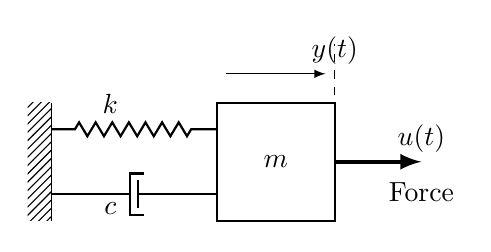
\begin{tikzpicture}[every node/.style={draw,outer sep=0pt,thick}]
    \tikzstyle{spring}=[thick,decorate,decoration={zigzag,pre length=0.3cm,post length=0.3cm,segment length=6}]
    \tikzstyle{damper}=[thick,decoration={markings,  
      mark connection node=dmp,
      mark=at position 0.5 with 
      {
        \node (dmp) [thick,inner sep=0pt,transform shape,rotate=-90,minimum width=15pt,minimum height=3pt,draw=none] {};
        \draw [thick] ($(dmp.north east)+(2pt,0)$) -- (dmp.south east) -- (dmp.south west) -- ($(dmp.north west)+(2pt,0)$);
        \draw [thick] ($(dmp.north)+(0,-5pt)$) -- ($(dmp.north)+(0,5pt)$) ; 
      }
    }, decorate]
    \tikzstyle{ground}=[fill,pattern=north east lines,draw=none,minimum width=0.75cm,minimum height=0.3cm]
    
    \node (M) [minimum width=1.5cm, minimum height=1.5cm] {$m$};
    \node (arrowstart) [name=arrowstart, above = 1cm of M.west,draw=none]{};
    \node (arrowend) [name=arrowend, above= 1cm of M.east,draw=none]{};
    
    \node (wall) [ground, rotate=-90, minimum width=1.5cm,yshift=-3cm] {};
    \draw (wall.north east) -- (wall.north west);
    
    % no need for ground, commented out
    % \node (gnd) [ground, rotate=0, minimum width=5cm,yshift=-0.9cm, xshift=-0.65cm] {};
    % \draw (wall.south east) -- (M.south east)--+(1.1cm,0);
    
    \draw [spring] (wall.160) -- ($(M.north west)!(wall.160)!(M.south west)$);
    \draw [damper] (wall.20) -- ($(M.north west)!(wall.20)!(M.south west)$);
    
    \draw [-latex,ultra thick] (M.east) ++ (0,0) -- +(1.1cm,0) node [above, draw=none]{$u(t)$} node [below=.15cm,draw=none]{Force};
    \draw [dashed] (M.east) ++ (0,0) -- +(0,1.5cm);
    \draw [-latex] (arrowstart) -- (arrowend) node[draw=none, above]{$y(t)$};
    
    \node[below=.3cm, draw=none] at (-2.1,-0.1){$c$};
    \node[above, draw=none] at (-2.1,0.5){$k$};
\end{tikzpicture}
\end{figure}
Impulse response: $g(t) = -e^{-\frac{1}{2}t}+ e^{-\frac{1}{3}t}$ with poles at $s=-\frac{1}{2}$, $s=-\frac{1}{3}$.\\\\
Recall that: The poles determine how quickly the system moves towards the steady state. Since $e^{-\frac{1}{2}t}$ decays faster than $e^{-\frac{1}{3}t}$, $s=-\frac{1}{3}$ is the dominant pole.\\\\
{\color{red}Dominant pole} lies closer to the imaginary axis in $s$-plane.
\begin{figure}[H] 
    \centering 
    \begin{tikzpicture}[>=latex]
    \begin{axis}[
      axis x line=center,
      axis y line=center,
      xtick = {-1/3, -1/2},
      xticklabels={$-\frac{1}{3}$, $-\frac{1}{2}$},
      yticklabels={,,},
      xlabel={$Re$},
      ylabel={$Im$},
      xlabel style={below right},
      ylabel style={above left},
      xmin=-0.6,
      xmax=0.2,
      ymin=-0.2,
      ymax=0.2,
      x=5cm, y=8cm/2]
    \addplot[
        scatter/classes={a={blue}, b={red}},
        scatter, mark=*, only marks, 
        scatter src=explicit symbolic 
    ] table [meta=class] {
        x y class
        -0.5 0 a 
        -0.333 0 b 
    };
    \end{axis}
\end{tikzpicture}
\end{figure}
\end{ex}
%----------------EXAMPLE END----------------%
%---------------EXAMPLE START---------------%
\begin{ex}{}
    Obtain the dominant pole approximation of $\displaystyle G(s) = \frac{10}{(s+10)(s^{2}+2s+2)}$\\\\
    Poles at $s=-10$ and $s = -1\pm j$. Since $s = -1\pm j$ lie closer to the imaginary axis, these are dominant poles of the system.
    \begin{figure}[H] 
        \centering 
        \begin{tikzpicture}[>=latex]
    \begin{axis}[
      axis x line=center,
      axis y line=center,
      xtick = {-3, -0.5},
      xticklabels={10, $-1\pm j$},
      yticklabels={},
      xlabel={$Re$},
      ylabel={$Im$},
      xlabel style={below right},
      ylabel style={above left},
      xmin=-3.2,
      xmax=0.2,
      ymin=-1.2,
      ymax=1.2,
      x=1cm, 
      y=2cm/2]
    \addplot[
        scatter/classes={a={blue}, b={red}},
        scatter, mark=*, only marks, 
        scatter src=explicit symbolic 
    ] table [meta=class] {
        x y class
        -0.5 0.6 b 
        -0.5 -0.6 b 
        -3 0 a
    };
    \end{axis}
\end{tikzpicture}
    \end{figure}
    We can approximate the system by 
    \begin{itemize}
    \item keeping only the dominant poles
    \item ensuring the equal steady state for unit step response
    \end{itemize}
    For the case above, since $s = -1\pm \mathbf{j}$ are the dominant poles:
    \[ G(s) = \frac{10}{(s+10)(s^{2}+2s+2)} \quad \to \quad \hat{G}(s) =\frac{K}{s^{2}+2s+2}\]
    To determine the value of $K$:
    \[\begin{cases}
    \displaystyle
    y(\infty) = \lim_{s\to 0}sY(s) = \lim_{s\to0}sG(s)\frac{1}{s} = \frac{1}{2} \quad \\
    \displaystyle
    \hat{y}(\infty) = \lim_{s\to 0}s\hat{Y}(s) = \lim_{s\to0}s\hat{G}(s)\frac{1}{s} = \frac{K}{2}\\
    \end{cases}\]
    $\therefore$ \quad $K = 1$.
\end{ex}
%----------------EXAMPLE END----------------%

%-------------------------------------------%
\subsection{Good and Bad Approximations}
%-------------------------------------------%
\begin{itemize}
    \item If the dominant poles are very different from the other poles, this will lead to a good approximation;
        \begin{ex}{}
            The system $\displaystyle G(s)=\frac{10}{(s+10)(s^{2}+2s+2)}$ has poles at $s = -10$, $s = -1 \pm \mathbf{j}$. \\\\Since poles are not close each other, the 2\textsuperscript{nd} order approximation is almost equivalent to the original system.
            \begin{figure}[H] \centering 
                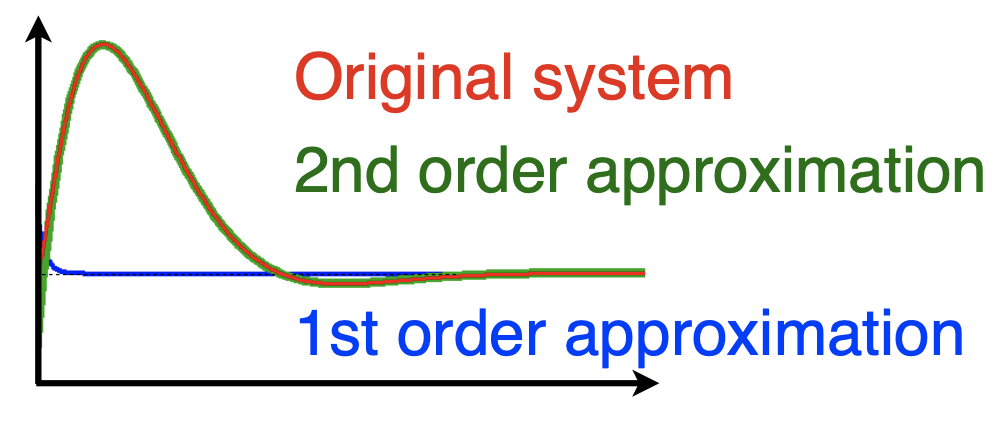
\includegraphics[width=.4\textwidth]{images/good_approx.png}
                \caption{A good approximation, $G(s)=\frac{10}{(s+10)(s^{2}+2s+2)}$}
            \end{figure}
        \end{ex}
    
    \item If the dominant pole is close to the other poles, the approximation will be imprecise.
    %---------------EXAMPLE START---------------%
        \begin{ex}{}
            The system $\displaystyle G(s)=\frac{1}{(s+51)(s^{2}+100s+9000)}$ has poles at $s = -51$, $s = -50 \pm 81\mathbf{j}$.\\\\ In this case, poles are close to each other, which leads to the bad approximation.
            \begin{figure}[H] 
                \centering 
                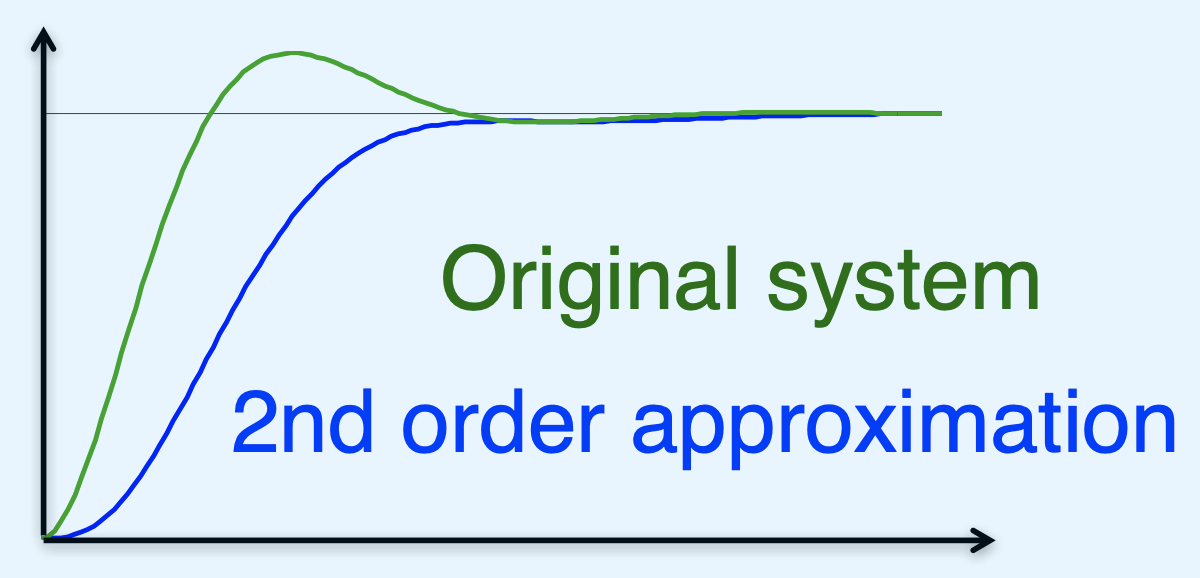
\includegraphics[width=.4\textwidth]{images/bad_approx.png}
                \caption{A bad approximation, $G(s)=\frac{1}{(s+51)(s^{2}+100s+9000)}$}
            \end{figure}
        \end{ex}
    %----------------EXAMPLE END----------------%
\end{itemize}
%-------------------------------------------%
\subsection{Time Response Analysis for 1\textsuperscript{st} Order Systems}
%-------------------------------------------%
\[
T\frac{dy(t)}{dt}+y(t)=Ku(t) 
\quad {\color{gray}\xleftrightarrow[\mathcal{L}^{-1}]{\mathcal{L}}} \quad  
(Ts+1)Y(s)=KU(s)
\]
\begin{itemize}
    \item The transfer function for a 1\textsuperscript{st} order system is $G(s)=\frac{K}{Ts+1}$ with poles at $s=-\frac{1}{T}$,  $T$ is known as the \textbf{time constant}. 
    \item Time constant determines how fast the system moves towards the steady state.
\end{itemize}

%-------------------------------------------%
\subsubsection{Impulse Response of 1\textsuperscript{st} Order Systems}
%-------------------------------------------%
\[
U(s)=1 
\quad {\color{gray}\longrightarrow} \quad 
\boxed{G(s)=\frac{K}{Ts+1}}
\quad {\color{gray}\longrightarrow} \quad 
Y(s)= \frac{K}{Ts+1} 
\quad {\color{gray}\xrightarrow[]{\mathcal{L}^{-1}}} \quad 
y(t) = \frac{K}{T}e^{-\frac{1}{T}t}
\]

\begin{figure}[H] 
    \centering 
    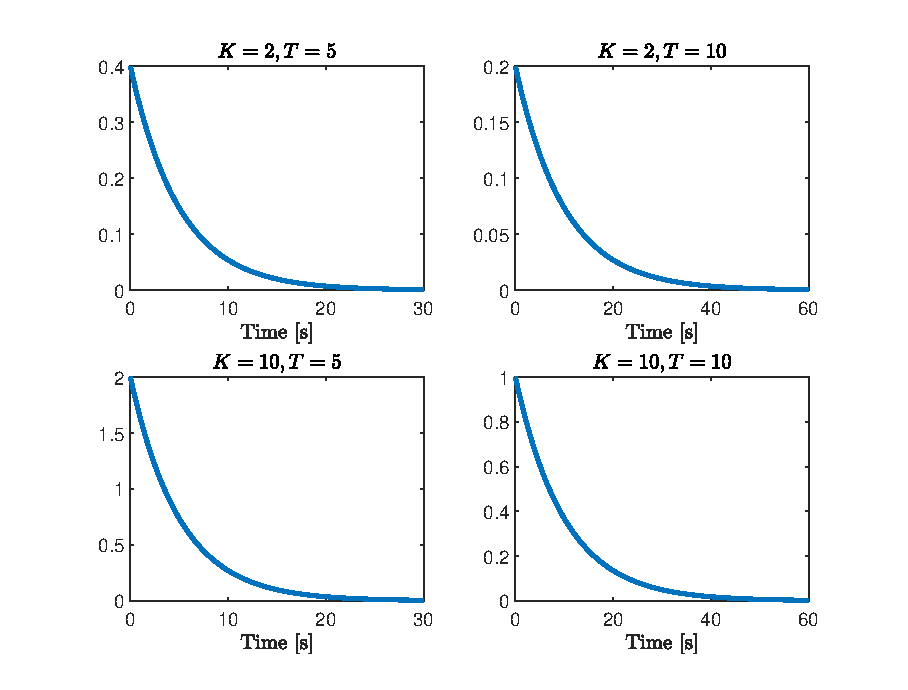
\includegraphics[width=.8\textwidth]{images/impulse_response.eps}
    \caption{Impulse response of 1\textsuperscript{st} order systems}
\end{figure}

%-------------------------------------------%
\subsubsection{Step Response of 1\textsuperscript{st} Order Systems}
%-------------------------------------------%
\[
U(s)=\frac{1}{s} 
\quad {\color{gray}\longrightarrow} \quad 
\boxed{G(s)=\frac{K}{Ts+1}} 
\quad {\color{gray}\longrightarrow} \quad  
Y(s)= \frac{1}{s}\frac{K}{Ts+1} 
\quad {\color{gray}\xrightarrow[]{\mathcal{L}^{-1}}} \quad  
y(t) = K(1-e^{-\frac{1}{T}t})
\]

\begin{figure}[H] 
    \centering 
    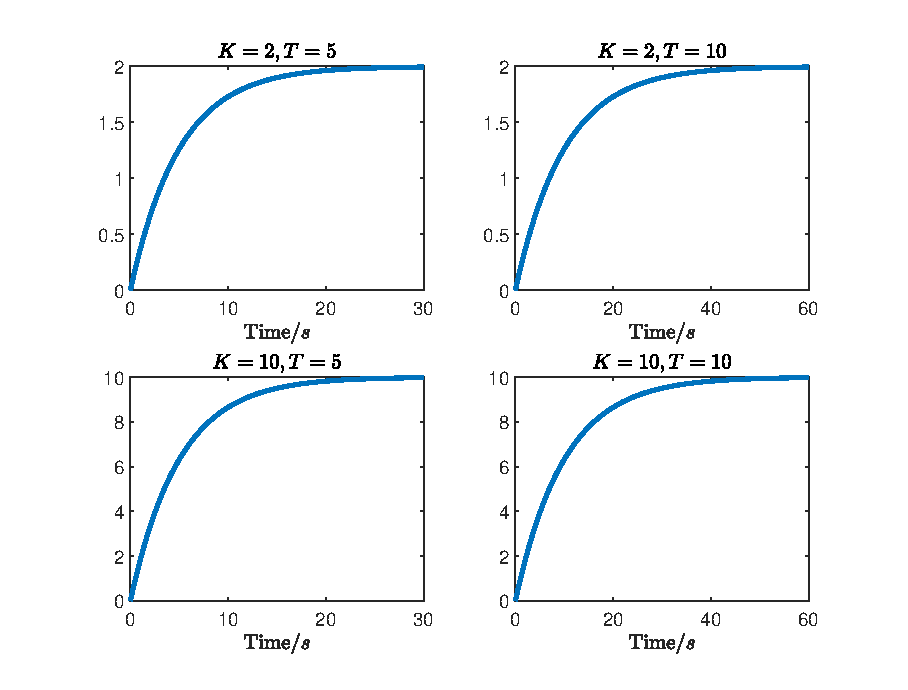
\includegraphics[width=.8\textwidth]{images/step_response.eps}
    \caption{Step response of 1\textsuperscript{st} order systems}
\end{figure}

%-------------------------------------------%
\subsection{Time Response Analysis for 2\textsuperscript{nd} Order Systems}
%-------------------------------------------%
\[\frac{d^{2}y(t)}{dt^{2}}+2\zeta\omega_{n}\frac{dy(t)}{dt}+\omega_{n}^{2}y(t) = K\omega_{n}^{2}u(t)\]
The transfer function for a $2^{nd}$ order system is $\displaystyle G(s)= \frac{K\omega_{n}^{2}}{s^{2}+2\zeta\omega_{n}s+\omega_{n}^{2}}$, where
\begin{itemize}
    \item $\zeta$ is \textbf{damping ratio}. It measures how much the system oscillates as the output decays towards the steady state.
    
    \item $\omega_{n}$ is \textbf{undamped natural frequency}. It measures how fast the system oscillates during the transient response.
\end{itemize}
Time response, $Y(s)$, of  $2^{nd}$ order systems:
\begin{itemize}
    \item Impulse response:\[Y(s)= \frac{K\omega_{n}^{2}}{s^{2}+2\zeta\omega_{n}s+\omega_{n}^{2}}\]
    
    \item Step response:\[Y(s)= \frac{K\omega_{n}^{2}}{s^{2}+2\zeta\omega_{n}s+\omega_{n}^{2}}\frac{1}{s}\]
\end{itemize}
The characteristic equations are both $s^{2}+2\zeta\omega_{n}s+\omega_{n}^{2}=0$, with poles at $s = (-\zeta\pm \sqrt{\zeta^{2}-1})\omega_{n}$.
This gives 3 cases: 
    \[
    s=\begin{cases}
    s = \pm\mathbf{j}\omega_{n}\ ,&\zeta = 0\\
    s = (-\zeta\pm \mathbf{j}\sqrt{1-\zeta^{2}})\omega_{n}\ , & 0<\zeta<1\\
    s = (-\zeta\pm \sqrt{\zeta^{2}-1})\omega_{n}\ , &\zeta>1\\
    \end{cases} 
    \]

%-------------------------------------------%
\subsubsection{\underline{Case 1:} $\zeta = 0$, Undamped Response}
%-------------------------------------------%
Undamped response happens when damping ratio $\zeta=0$, with poles at $s = \pm \mathbf{j}\omega_{n}$.
The undamped step response is \textbf{purely sinusoidal}:
\[
Y(s) = \frac{K\omega_{n}^{2}}{s^{2}	+2\zeta\omega_{n}s+\omega_{n}^{2}}\frac{1}{s}
\quad  {\color{gray}\xrightarrow{\mathcal{L}^{-1}}} \quad
y(t) = K(1-\cos(\omega_{n}t)) 
\]

\begin{figure}[H] 
    \centering 
    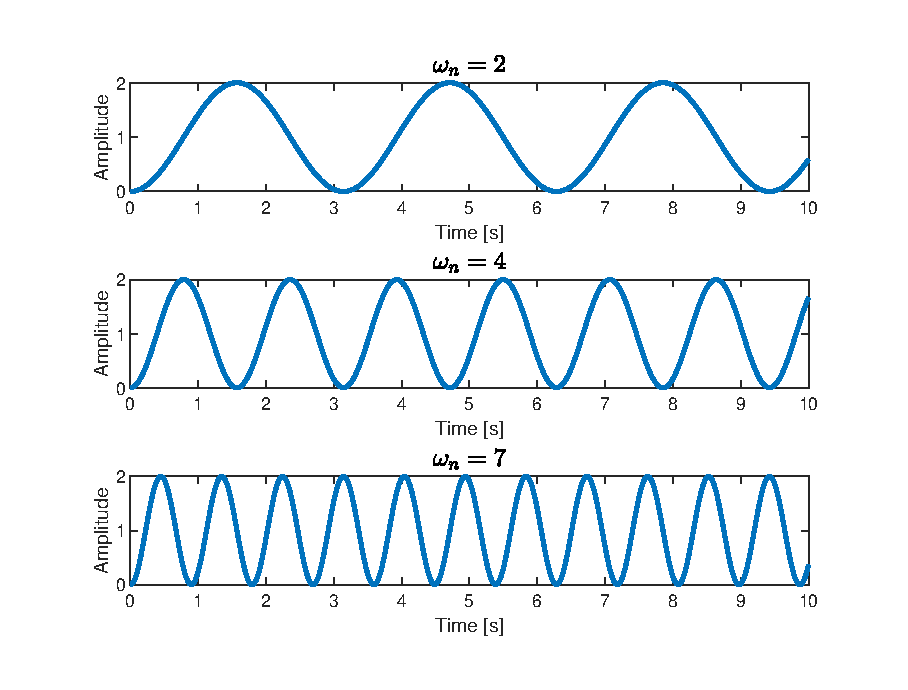
\includegraphics[width=.8\textwidth]{images/undamped_response.eps}
    \caption{Undamped response of 2\textsuperscript{nd} order systems. $K=1$}
\end{figure}

%-------------------------------------------%
\subsubsection{\underline{Case 2:} $0<\zeta<1$, Underdamped Response}
%-------------------------------------------%
Underdamped response happens when damping ratio $0<\zeta<1$, with 2 conjugate poles at $s = (-\zeta\pm \mathbf{j} \sqrt{1-\zeta^{2}})\omega_{n}$.\\\\
The underdamped step response is \textbf{the combination of exponential function and sinusoidal function}:
\begin{itemize}
    \item Step response: 
    \[
    Y(s) = \frac{K\omega_{n}^{2}}{s^{2}	+2\zeta\omega_{n}s+\omega_{n}^{2}} \frac{1}{s} = K(\frac{1}{s}-\frac{s+\zeta\omega_{n}}{(s+\zeta\omega_{n})^{2}+\omega_{d}^{2}}-\frac{\zeta\omega_{n}}{(s+\zeta\omega_{n})^{2}+\omega_{d}^{2})})
    \]
    
    \item Take inverse Laplace transform:
    \[ {\color{gray}\xrightarrow{\mathcal{L}^{-1}}} \quad
    y(t) = K \bigg[ 1-\frac{e^{-\zeta\omega_{n} t}}{\sqrt{1-\zeta^{2}}} \sin(\omega_{d}t +\tan^{-1}\frac{\sqrt{1-\zeta^{2}}}{\zeta}) \bigg] 
    \]
    \begin{itemize}
        \item $\zeta\omega_{n}$ is known as \textbf{decay time constant};
        
        \item $\omega_{d}$ is known as \textbf{damped natural frequency} with the expression:
        \[\omega_{d} = \omega_{n}\sqrt{1-\zeta^{2}}\]
    \end{itemize}
\end{itemize}

\begin{figure}[H] 
    \centering 
    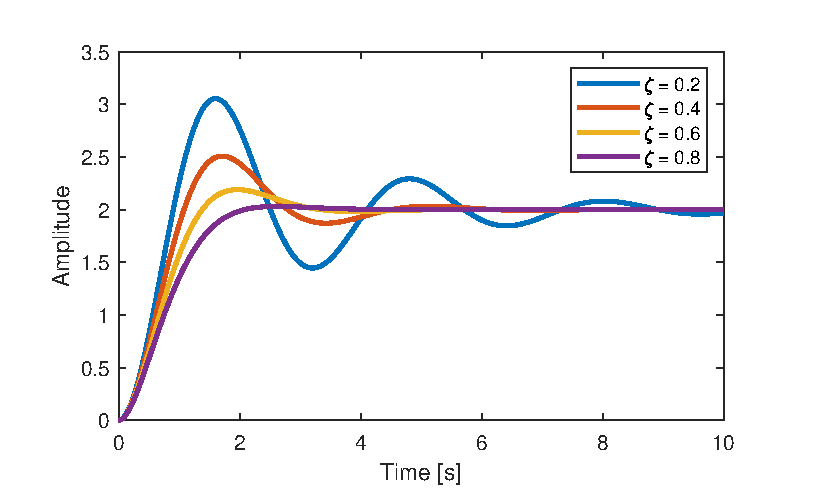
\includegraphics[width=.8\textwidth]{images/underdamped_response.eps}
    \caption{Underdamped response of 2\textsuperscript{nd} order systems. $\omega_{n}=2$, $K=2$}
\end{figure}

%-------------------------------------------%
\subsubsection{\underline{Case 3:} $\zeta>1$, Overdamped Response}
%-------------------------------------------%
Overdamped response happens when damping ratio $\zeta>1$, with 2 negative, real poles at $s = (-\zeta\pm \sqrt{\zeta^{2}-1})\omega_{n}$ which are refer as $\alpha$ and $\beta$.\\\\
The overdamped step response \textbf{quickly converges to a stable value}:
\begin{itemize}
    \item Step response:
    \[
    Y(s) = \frac{K\omega_{n}^{2}}{(s-\alpha)(s-\beta)} \frac{1}{s} = \frac{K\alpha\beta}{s(s-\alpha)(s-\beta)} = K\bigg[ \frac{1}{s}+\frac{1}{\alpha-\beta}(\frac{\beta}{s-\alpha}-\frac{\alpha}{s-\beta})\bigg]
    \]
    
\item Take inverse Laplace transform:
    \[
    {\color{gray}\xrightarrow{\mathcal{L}^{-1}}} \quad
    y(t) = K\bigg(1+\frac{\beta e^{\alpha t}-\alpha e^{\beta t}}{2\omega_{n}\sqrt{\zeta^{2}-1}}\bigg)
    \]
\end{itemize}

\begin{figure}[H] 
    \centering 
    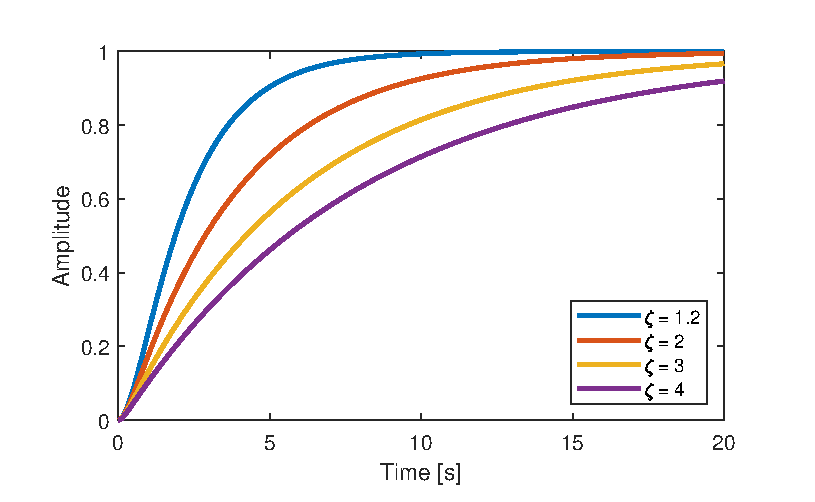
\includegraphics[width=.8\textwidth]{images/overdamped_response.eps}
    \caption{Overdamped response of 2\textsuperscript{nd} order systems. $\omega_{n}=1$, $K=1$}
\end{figure}

%-------------------------------------------%
\subsection{Transient Specification of 2\textsuperscript{nd} Order Systems}
%-------------------------------------------%
\begin{figure}[H] 
    \centering
    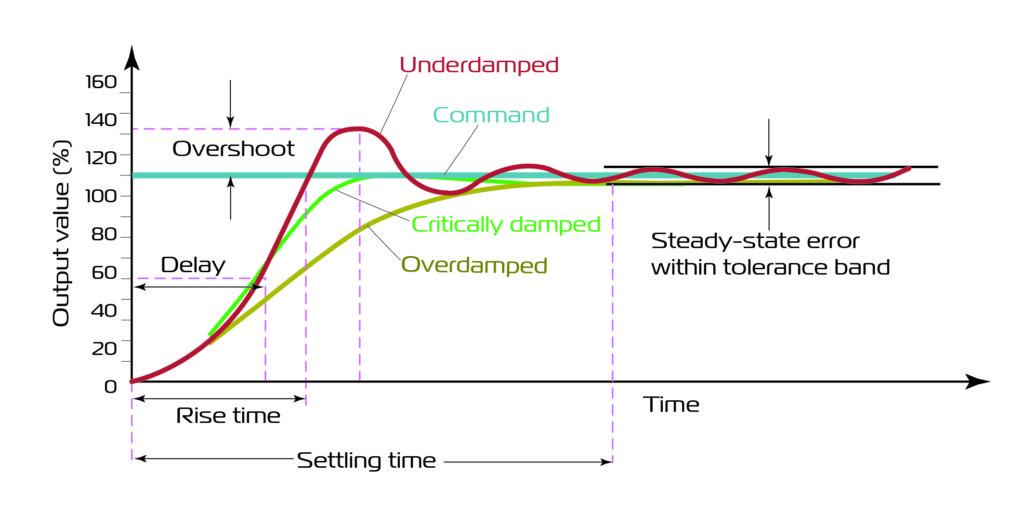
\includegraphics[width=0.8\textwidth]{images/PID_response.jpg}
    \caption{Overshoot, Rise time, Setting time and Steady-state error $^{1}$}
\end{figure}

\begin{itemize}
    \item \textbf{Rise time, $t_{r}$:} the time taken for the output to go from 10\% to 90\% of the final value.
    \[t_{r} = \frac{\pi-\cos^{-1}\zeta}{\omega_{d}}\]
    
    \item \textbf{Peak time, $t_{p}$:} the time taken for the output to reach its maximum value.
    \[t_{p} = \frac{\pi}{\omega_{n}\sqrt{1-\zeta^{2}}}\]
    
    \item \textbf{2\% Settling time, $t_{s2\%}$:} the time taken for the signal to be bounded to within a tolerance of x\% (here, 2\%) of the steady state value.
    \[t_{s2\%} = \frac{4}{\zeta\omega_{n}}\]
    
    \item \textbf{Overshoot}: 
    \[\textbf{overshoot} = \frac{\text{max value - min value}}{\text{final value}}\times 100\]
    
    \item \textbf{Steady-state error}: the difference between the input step value and the final value.
\end{itemize}

\footnotetext[1]{Reference \url{http://www.mee.tcd.ie/~corrigad/3c1/control_ho2_2012_students.pdf}}

%-------------------------------------------%
\newpage
\section{PID Control}
%-------------------------------------------%

%-------------------------------------------%
\subsection{Open-loop Control} 
%-------------------------------------------%
\begin{itemize}
    \item No feedback in open-loop control, output has no effect on the control action;
    
    \item Open-loop control is convenient when it is hard to measure output;
    
    \item It is only used if the uncontrolled plant dynamics is \textbf{perfectly known} and is not subject to any environmental changes.
\end{itemize}

\begin{figure}[H] 
    \centering 
    % 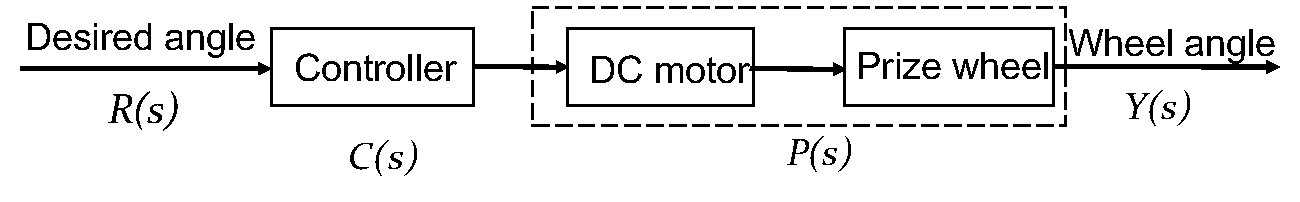
\includegraphics[width=.7\textwidth]{images/open-loop.pdf}
    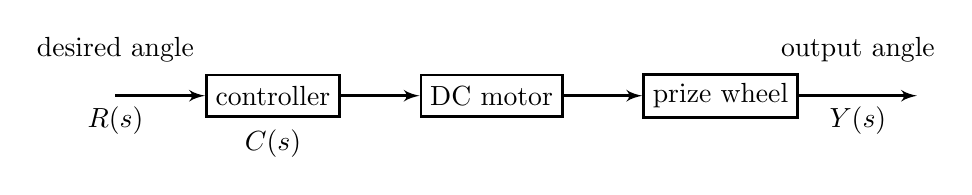
\begin{tikzpicture}[auto, node distance=2cm,>=latex',line width=1pt]
    \node [input, name=input] {};
    \node [block, right of=input] (controller1) {controller};
    \node [block, right= 1cm of controller1] (controller2) {DC motor};
    \node [block, right= 1cm of controller2] (controller3) {prize wheel};
    \node [output, right=1.5cm of controller3] (output) {};
    
    
    \draw [->] node[below]{$R(s)$} node[above=0.3cm]{desired angle}(input) --  (controller1)node [below=0.3cm]{$C(s)$};
    \draw [->] (controller1) -- (controller2);
    \draw [->] (controller2) -- (controller3);
    \draw [->] (controller3) -- node[below]{$Y(s)$} node[above=0.3cm]{output angle} (output);
\end{tikzpicture}
    \caption{Open-loop control system for a prize wheel}
\end{figure}
If we want the output follows the desired input, \textit{i.e.} $Y(s)=R(s)$, this is achievable by choosing the controller as $C(s) = P^{-1}(s)$.

%-------------------------------------------%
\subsection{On-off (bang-bang) Control}
%-------------------------------------------%
\begin{itemize}
    \item On-off control is the simplest closed-loop feedback control
    \item On-off control may cause oscillating errors due to the frequent switchings.
    \item Potential high input to the plant and wear-and-tear of the system.
\end{itemize}

\begin{figure}[H] 
    \centering 
    % 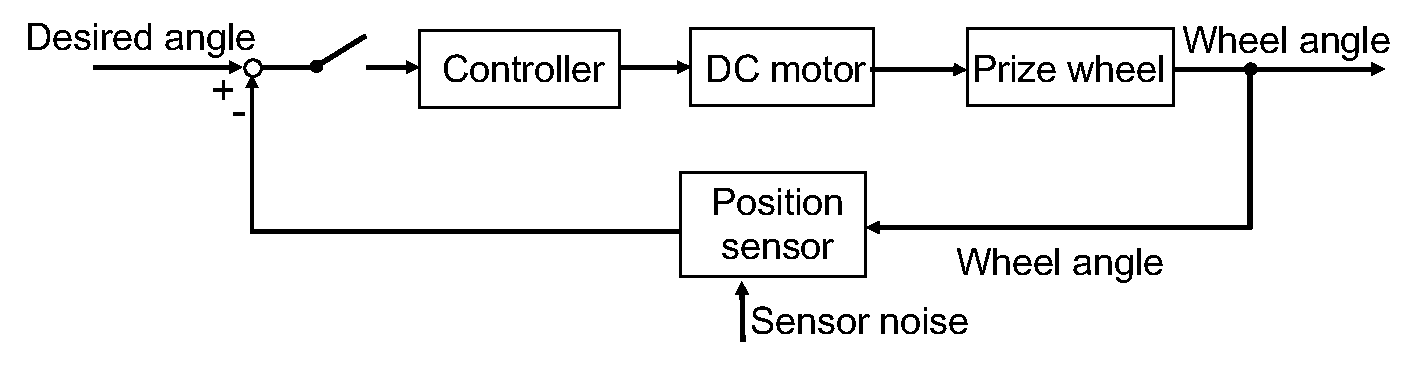
\includegraphics[width=.7\textwidth]{images/onoff.pdf}
    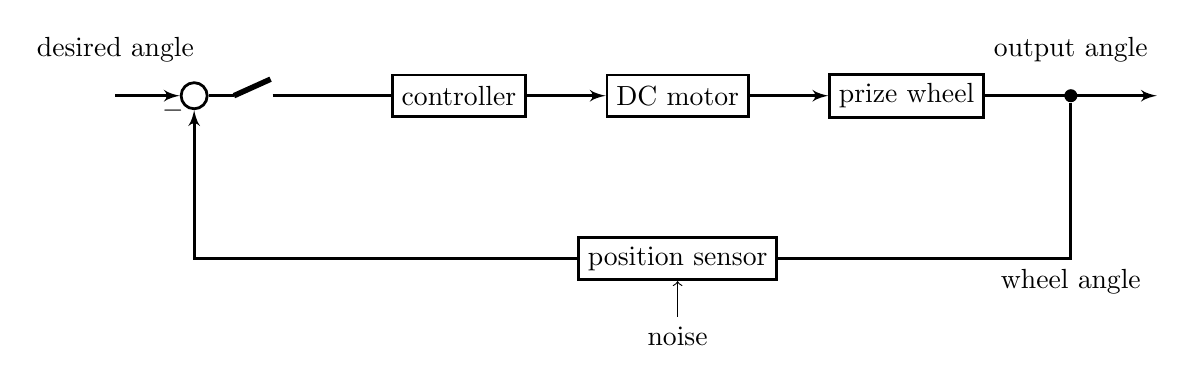
\begin{tikzpicture}[auto, node distance=1.5cm,>=latex',line width=1pt]
    \node [input, name=input] {};
    \node [sum, right of=input] (sum) {};
    \coordinate[right of = sum](switch){};
    \node [block, right= 1cm of switch] (controller1) {controller};
    \node [block, right= 1cm of controller1] (controller2) {DC motor};
    \node [block, right= 1cm of controller2] (controller3) {prize wheel};
    \coordinate [right=1cm of controller3, circle, scale=0.5, fill](tooutput){};
    \node [output, right=1cm of tooutput] (output) {};
    \coordinate [below= 0.2cm of tooutput] (measurements) {};
    \node[block, below= 1.5cm of controller2, pin={[pinstyle]below:noise}, node distance=3cm](controller4){position sensor};

    \draw [->] node[above=0.3cm]{desired angle}(input) -- (sum);
    \draw [-] (sum) to[normal open switch] (switch)-- (controller1);
    \draw [->] (controller1) -- (controller2);
    \draw [->] (controller2) -- (controller3);
    \draw [->] (controller3) -- node[above=0.3cm]{output angle} (output);
    \draw [-] (controller3) -- (tooutput) |- node[]{wheel angle}(controller4);
    \draw [->] (controller4) -| node[pos=1]{$-$} (sum);
\end{tikzpicture}

    \caption{On-off control system for a prize wheel}
\end{figure}
Take the example of the prize wheel. Position sensor measures the output angle, and compare this angle with the desired angle. Then use the switch\textit{(on-off)} to control the strength of the DC motor.

%-------------------------------------------%
\subsection{Gain (proportional) Control}
%-------------------------------------------%
\begin{itemize}
    \item Gain control applies control input that is proportional to the current error.
    \item It has very quick reaction to the current error
    \item But it is possible to \textbf{overshoot} when the error is magnified too much.
    \item Also, gain control leads to a non-zero \textbf{steady-state error}.
\end{itemize}

\begin{figure}[H] 
    \centering 
    % 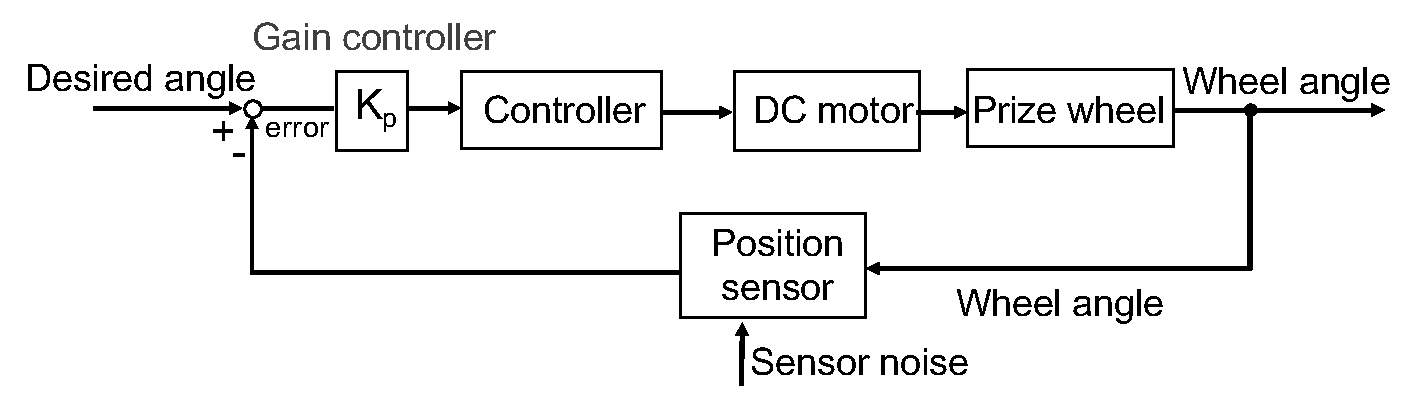
\includegraphics[width=.7\textwidth]{images/gain.pdf}
    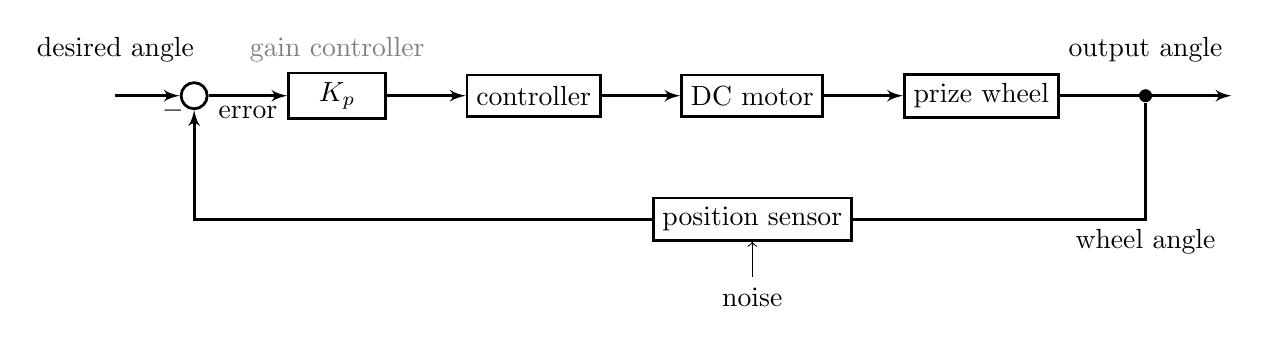
\begin{tikzpicture}[auto, node distance=1.5cm,>=latex',line width=1pt]
    \node [input, name=input] {};
    \node [sum, right of=input] (sum) {};
    \node [block, right= 1cm of sum] (controller) {$K_{p}$};
    \node [block, right= 1cm of controller] (controller1) {controller};
    \node [block, right= 1cm of controller1] (controller2) {DC motor};
    \node [block, right= 1cm of controller2] (controller3) {prize wheel};
    \coordinate [right=1cm of controller3, circle, scale=0.5, fill](tooutput){};
    \node [output, right=1cm of tooutput] (output) {};
    \coordinate [below= 1.5cm of tooutput] (measurements) {};
    \node[block, below= 1cm of controller2, pin={[pinstyle]below:noise}, node distance=3cm](controller4){position sensor};

    \draw [->] node[above=0.3cm]{desired angle}(input) -- (sum);
    \draw [->] (sum) -- node[below]{error}(controller) node[above=.3cm]{{\color{gray} gain controller}};
    \draw [->] (controller) -- (controller1);
    \draw [->] (controller1) -- (controller2);
    \draw [->] (controller2) -- (controller3);
    \draw [->] (controller3) -- node[above=0.3cm]{output angle} (output);
    \draw [-] (controller3) -- (tooutput) |- node[]{wheel angle}(controller4);
    \draw [->] (controller4) -| node[pos=1]{$-$} (sum);
\end{tikzpicture}

    \caption{Gain control system for a prize wheel}
\end{figure}

Take the example of the prize wheel. The position sensor measures the wheel angle and compare it with the desired angle. The error is then calculated and sent into the gain controller. The gain controller magnifies the error and send to the DC motor for further action. 

%-------------------------------------------%
\subsection{PID Control}
%-------------------------------------------%
PID control is the most common controller used in industry which aims to reduce the tracking error between desired and measured output of the system.

\begin{figure}[H] 
    \centering 
    % 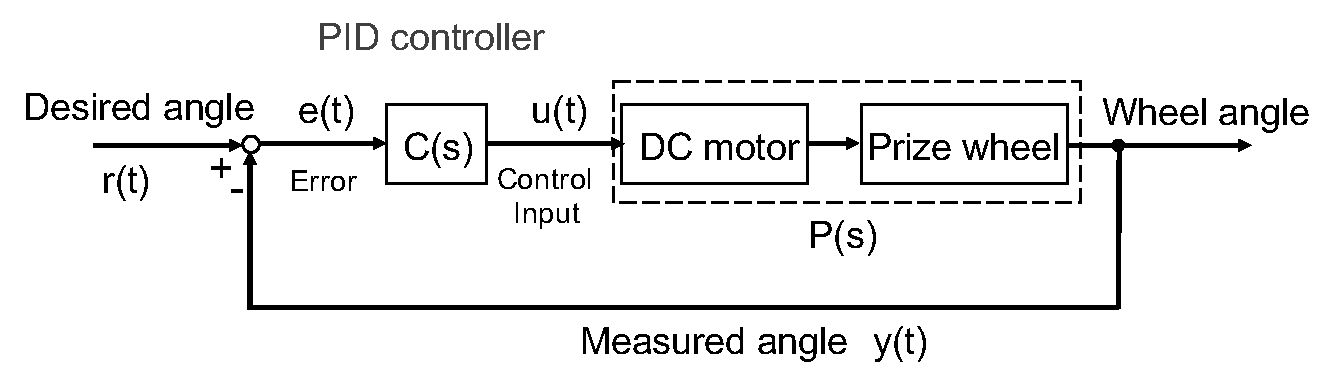
\includegraphics[width=.9\textwidth]{images/PID_control.pdf}
    % TikZ - PID controller

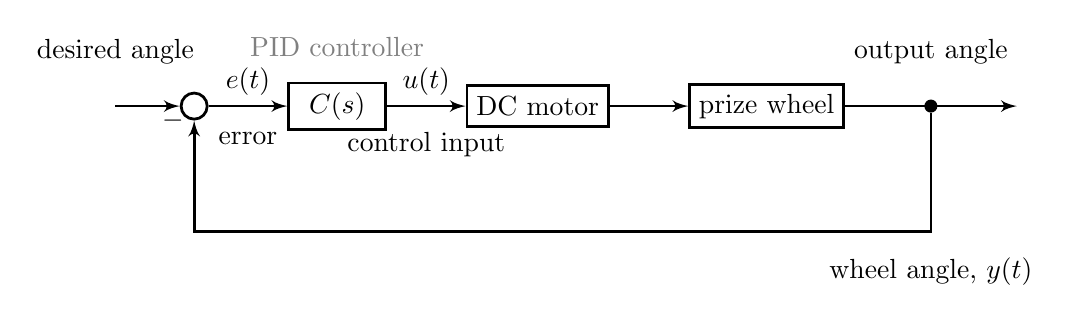
\begin{tikzpicture}[auto, node distance=1.5cm,>=latex',line width=1pt]
    \node [input, name=input] {};
    \node [sum, right of=input] (sum) {};
    \node [block, right= 1cm of sum] (controller1) {$C(s)$};
    \node [block, right= 1cm of controller1] (controller2) {DC motor};
    \node [block, right= 1cm of controller2] (controller3) {prize wheel};
    \coordinate [right=1cm of controller3, circle, scale=0.5, fill](tooutput){};
    \node [output, right=1cm of tooutput] (output) {};
    \coordinate [below= 1.5cm of tooutput] (measurements) {};

    \draw [->] node[above=0.4cm]{desired angle}(input) -- (sum);
    \draw [->] (sum) -- node[below=.2cm]{error} node[above]{$e(t)$}(controller1) node[above=.5cm]{{\color{gray} PID controller}};
    \draw [->] (controller1) -- node[below=.2cm]{control input} node[above]{$u(t)$}(controller2);
    \draw [->] (controller2) -- (controller3);
    \draw [->] (controller3) -- node[above=0.4cm]{output angle} (output);
    \draw [->] (controller3) -- (tooutput) |- (measurements) node[below=.2cm]{wheel angle, $y(t)$} -|  node[pos=1]{$-$} (sum);
\end{tikzpicture}
    \caption{PID control system for a prize wheel}
\end{figure}

\begin{itemize}
    \item Control input is the sum of \textbf{\underline{P}roportional}, \textbf{\underline{I}ntegral} and \textbf{\underline{D}erivative} of the error.
    
    \item Control input can be represented as:
    \[
    u(t) = K_{P}\  e(t)+K_{I}\int_{0}^{t}e(\tau)\mathrm{d}\tau + K_{D}\frac{\mathrm{d}e(t)}{\mathrm{d}t}
    \]
    
    \item PID controller can be represented as:
    \[C(s) =K_{P}+\frac{K_{I}}{s}+K_{D}s \]
    
        \begin{itemize}
             \item $K_{P}$ stands for \textbf{proportional gain}. It uses the information from the \textit{present error}.
             \item $K_{I}$ stands for \textbf{integral gain}. It uses the information from the \textit{past error}.
             It removes the steady-state error.
             \item $K_{P}$ stands for \textbf{derivative gain}. It uses the \textit{future error}. It improves the stability but has no effect on steady-state error.
        \end{itemize}
\end{itemize}

%-------------------------------------------%
\subsubsection{System response to $K_{P}$, $K_{I}$ and $K_{D}$}
%-------------------------------------------%
\begin{table}[H] \centering
    \begin{tabular}{|c|c|c|c|c|} \hline
        \textbf{Increase of} &\textbf{Overshoot}& \textbf{Rise Time} &\textbf{Settling Time}& \textbf{Steady-state error}\\ \hline
        $K_{P}$&Increase&  Decrease& Small increase& Decrease\\ \hline
        $K_{I}$&Increase &Decrease& Increase& Eliminate\\ \hline
        $K_{D}$&Decrease& Decrease& Decrease& No impact\\ \hline
    \end{tabular}
\end{table}

\begin{figure}[H] 
    \centering
    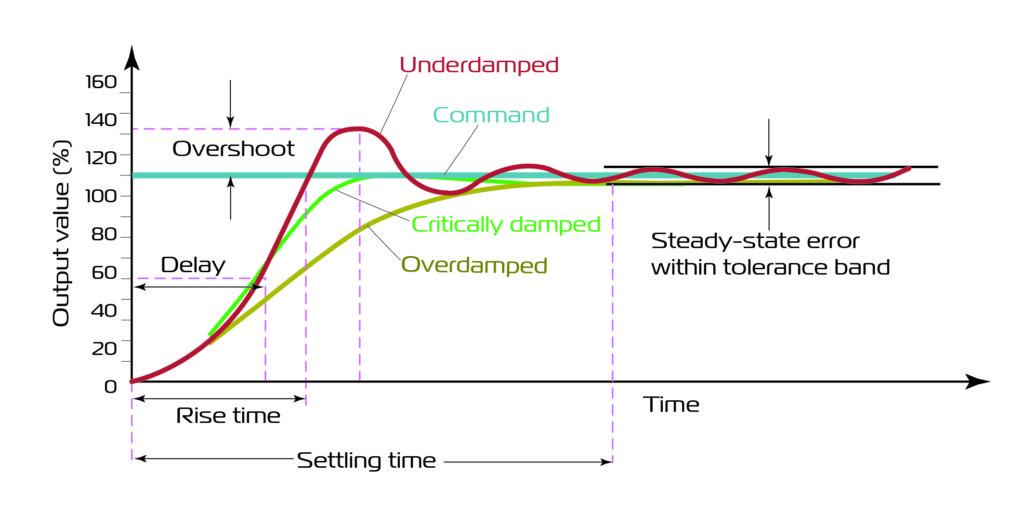
\includegraphics[width=0.8\textwidth]{images/PID_response.jpg}
\end{figure}

\newpage
\section{Bode Plots}
Bode plots are used to evaluate the behaviour of closed-loop systems.
\begin{itemize}
    \item \textbf{Gain plot} 
    \[
        20\log_{10}\lvert G(j\omega) \rvert \ \text{\textcolor{gray}{[in dB]}}\quad \text{v.s.} \quad \omega \ \textcolor{gray}{(\text{in } \log_{10} \ \text{scale})}
    \]
    
    \item \textbf{Phase plot} 
    \[
        \angle G(j\omega) \ \text{\textcolor{gray}{[in deg]}} \quad \text{v.s.} \quad \omega \ \textcolor{gray}{(\text{in } \log_{10} \ \text{scale})}  
    \]
\end{itemize}
The Bode plots of a complex system can be obtained by the addition of Bode plots for simple systems.
\begin{itemize}
    \item For gain plot:
    \[
        20\log_{10}\lvert G(j\omega)\rvert  = 20\log_{10}\lvert G_{1}(j\omega)\rvert+20\log_{10}\lvert G_{2}(j\omega)\rvert
    \]
    
    \item For phase plot:
    \[
        \angle G(j\omega) = \angle G_{1}(j\omega)+\angle G_{2}(j\omega)
    \]
\end{itemize}

\subsection{Bode Plots for Constant Gain, $G(s) = K$}
\begin{itemize}
    \item \textbf{Gain plot}: $20\log_{10}\lvert G(j\omega) \rvert \ = 20\log_{10}K$ 
    \item \textbf{Phase plot}: $\angle G(j\omega) = 0^{\circ}$
\end{itemize}

\begin{figure}[H] 
    \centering 
    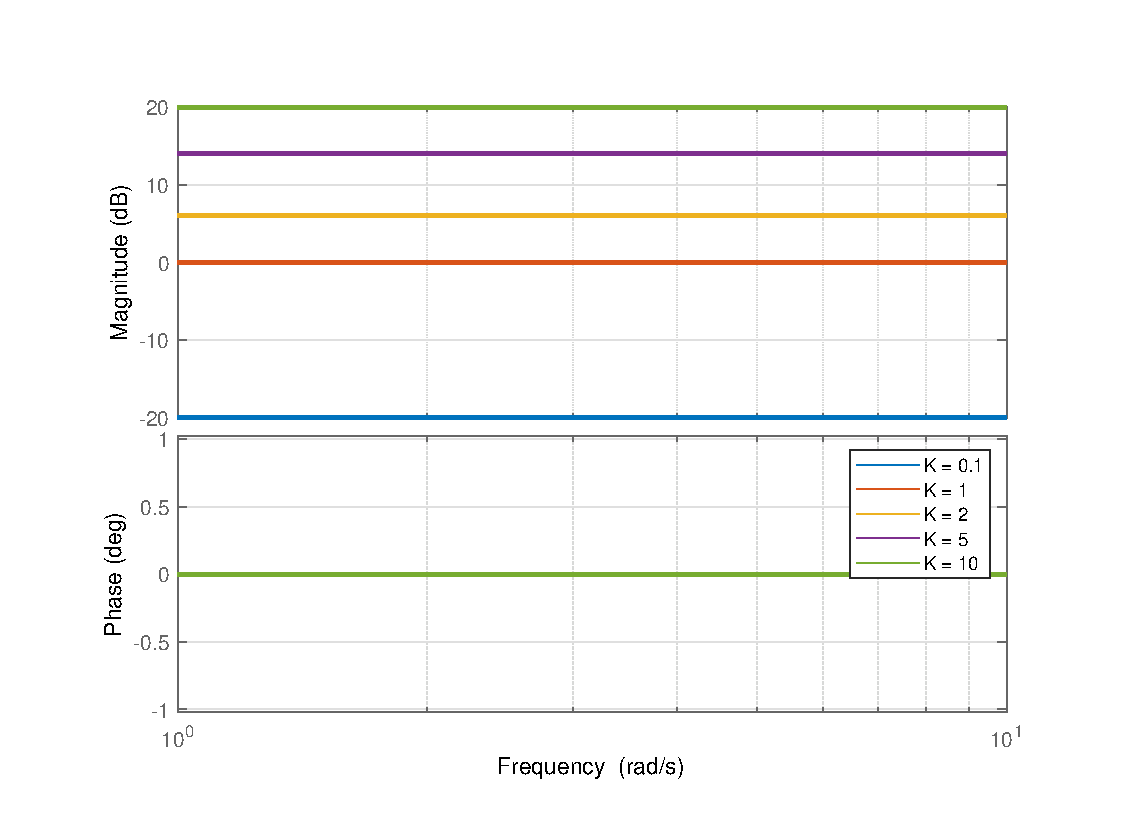
\includegraphics[width=.7\textwidth]{images/bode5.eps}
    \caption{Bode plot of $G(s) = K$. Magnitude plot is a constant.}
\end{figure}

\subsection{Bode Plots for Differentiator, $G(s) = s^{n}$}
\begin{itemize}
    \item \textbf{Gain plot}: 
    \[
        20\log_{10}\lvert G(j\omega) \rvert  = 20\log_{10}\lvert (j\omega)^{n} \rvert = n\cdot 20\log_{10}\lvert (j\omega) \rvert=\boxed{n\cdot20\log_{10}\omega}
    \]
    
    \item \textbf{Phase plot}: $\angle G(j\omega) = \angle (j\omega)^{n} = \boxed{n\cdot 90^{\circ}}$
    
    \item Gain difference $\Delta$ over the interval $[\omega_{1}, \omega_{2}] $: 
    \[
        \Delta = n\cdot20(\log_{10}\omega_{1}-\log_{10}\omega_{2})=\boxed{n\cdot20 \log_{10}\frac{\omega_{1}}{\omega_{2}}}
    \]
    This gives the slope$=n\cdot 20$ \textcolor{gray}{[dB/decade]}
\end{itemize}

\begin{figure}[H] 
    \centering 
    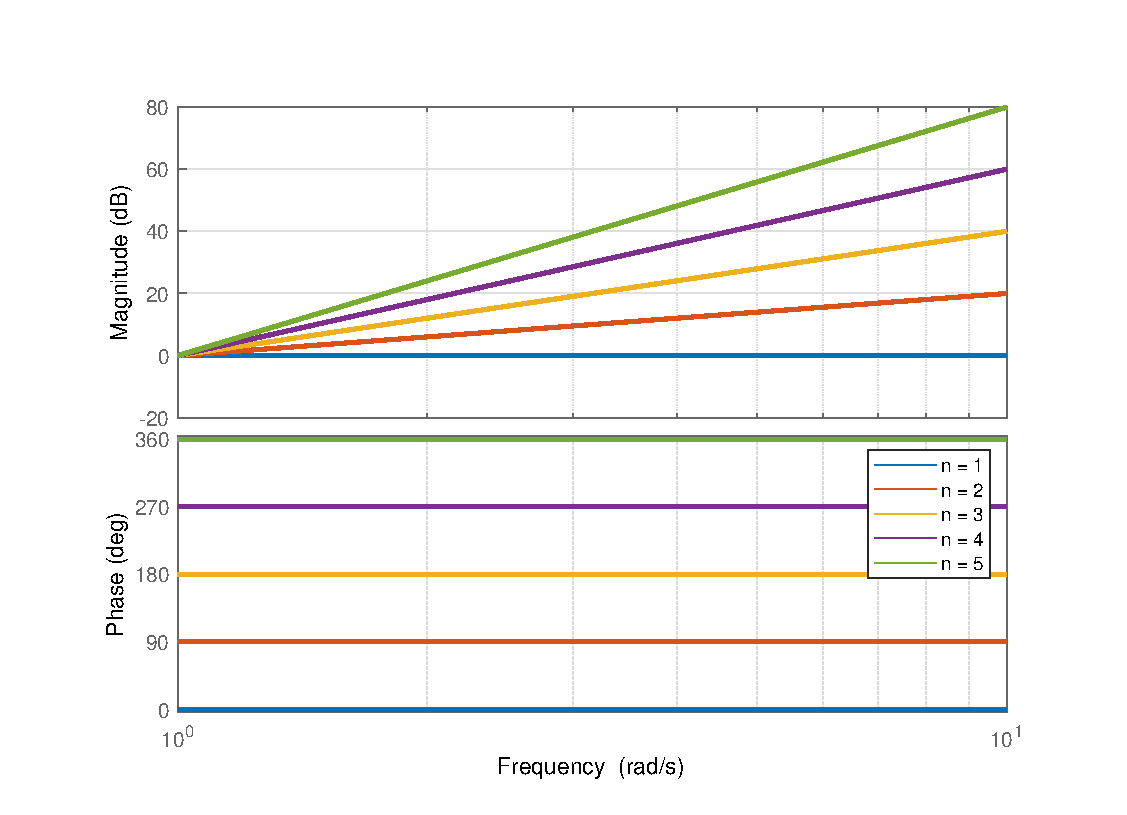
\includegraphics[width=.7\textwidth]{images/bode6.eps}
    \caption{Bode plot of $G(s) = s^{n}$.}
\end{figure}

\subsection{Bode Plots for Integrator, $G(s) = (\frac{1}{s})^{n}$}
\begin{itemize}
    \item \textbf{Gain plot}:
    \[
        20\log_{10}\lvert G(j\omega) \rvert
        = 20 \log_{10} \lvert (\frac{1}{j\omega})^{n} \rvert 
        = -n \cdot 20 \log_{10} \lvert (j\omega) \rvert
        = \boxed{-n\cdot20\log_{10}\omega}
    \]
    
    \item \textbf{Phase plot}: $\angle G(j\omega) = \angle (\frac{1}{j\omega})^{n} = \boxed{-n\cdot 90^{\circ}}$
    
    \item Gain difference $\Delta$ over the interval $[\omega_{1}, \omega_{2}] $: 
    \[ 
        \Delta = -n\cdot20(\log_{10}\omega_{1}-\log_{10}\omega_{2})=\boxed{-n\cdot20 \log_{10}\frac{\omega_{1}}{\omega_{2}}}
    \]
    This gives the slope$=-n\cdot 20$ \textcolor{gray}{[dB/decade]}
\end{itemize}

\begin{figure}[H] 
    \centering 
    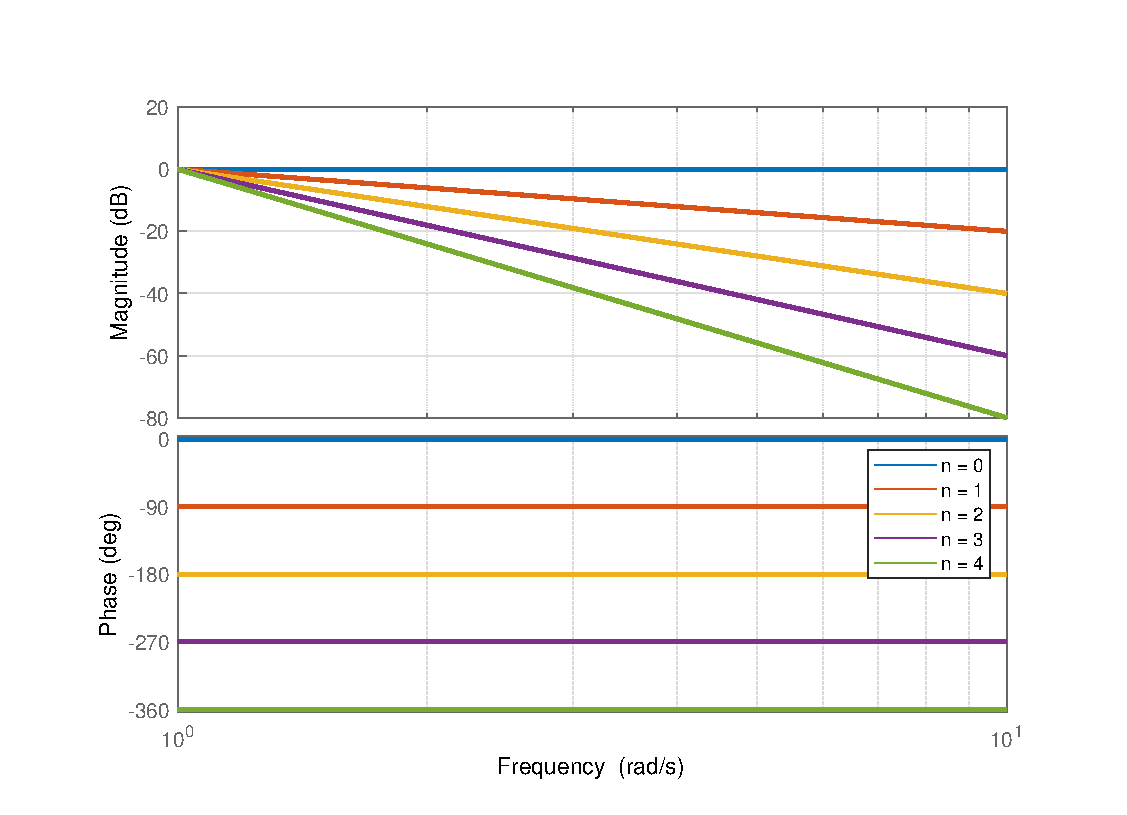
\includegraphics[width=.7\textwidth]{images/bode4.eps}
    \caption{Bode plot of  $G(s) = (\frac{1}{s})^{n}$.}
\end{figure}

\subsection{Bode Plots for 1\textsuperscript{st} Order System, $G(s) = \frac{K}{Ts+1}$}
\begin{itemize}
    \item \textbf{Gain plot}: 
    \begin{align*}
    \begin{split}
    20 \log_{10} \lvert G(j\omega) \rvert  
    & = 20\log_{10} \lvert \frac{K}{Ts+1} \rvert 
    = 20\log K-20\log\sqrt{T^{2}\omega^{2}+1} \\
    & \approx 
    \begin{cases} 
        20 \log K                   & T\omega<<1\\
        20 \log K - 20\log T\omega  & T\omega>>0
    \end{cases} 
    \end{split} 
    \end{align*}
    
    \item \textbf{Phase plot}: 
    \[
        \angle G(j\omega) \= \angle \frac{1}{Tj\omega+1}=\frac{-T\omega j +1}{T^{2}\omega^{2}+1}=\tan^{-1}(-T\omega)\approx 
        \begin{cases}
            0^{\circ}   & T\omega<<1\\
            -45^{\circ} & \omega=\omega_{c}=\frac{1}{T}\\
            -90^{\circ} & T\omega>>0
        \end{cases}
    \]
    
    \item Gain difference $\Delta$ over the interval $[\omega_{1}, \omega_{2}] $: \[ \Delta = -20(\log_{10}\omega_{1}-\log_{10}\omega_{2})=\boxed{-20 \log_{10}\frac{\omega_{1}}{\omega_{2}}}\]
    This gives the slope$=- 20$ \textcolor{gray}{[dB/decade]}
    
    \item Corner frequency: $20\log T\omega_{c}=0 \to \omega_{c} = \frac{1}{T}$

    \begin{figure}[H] 
        \centering 
        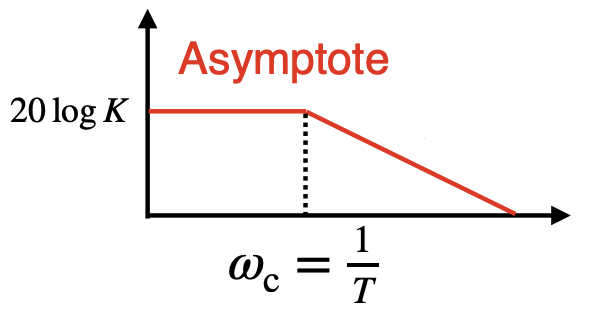
\includegraphics[width=.3\textwidth]{images/corner_1.png}
        \caption{Corner frequency, $\omega_{c}$}
    \end{figure}
    
    \begin{figure}[H]
        \centering 
        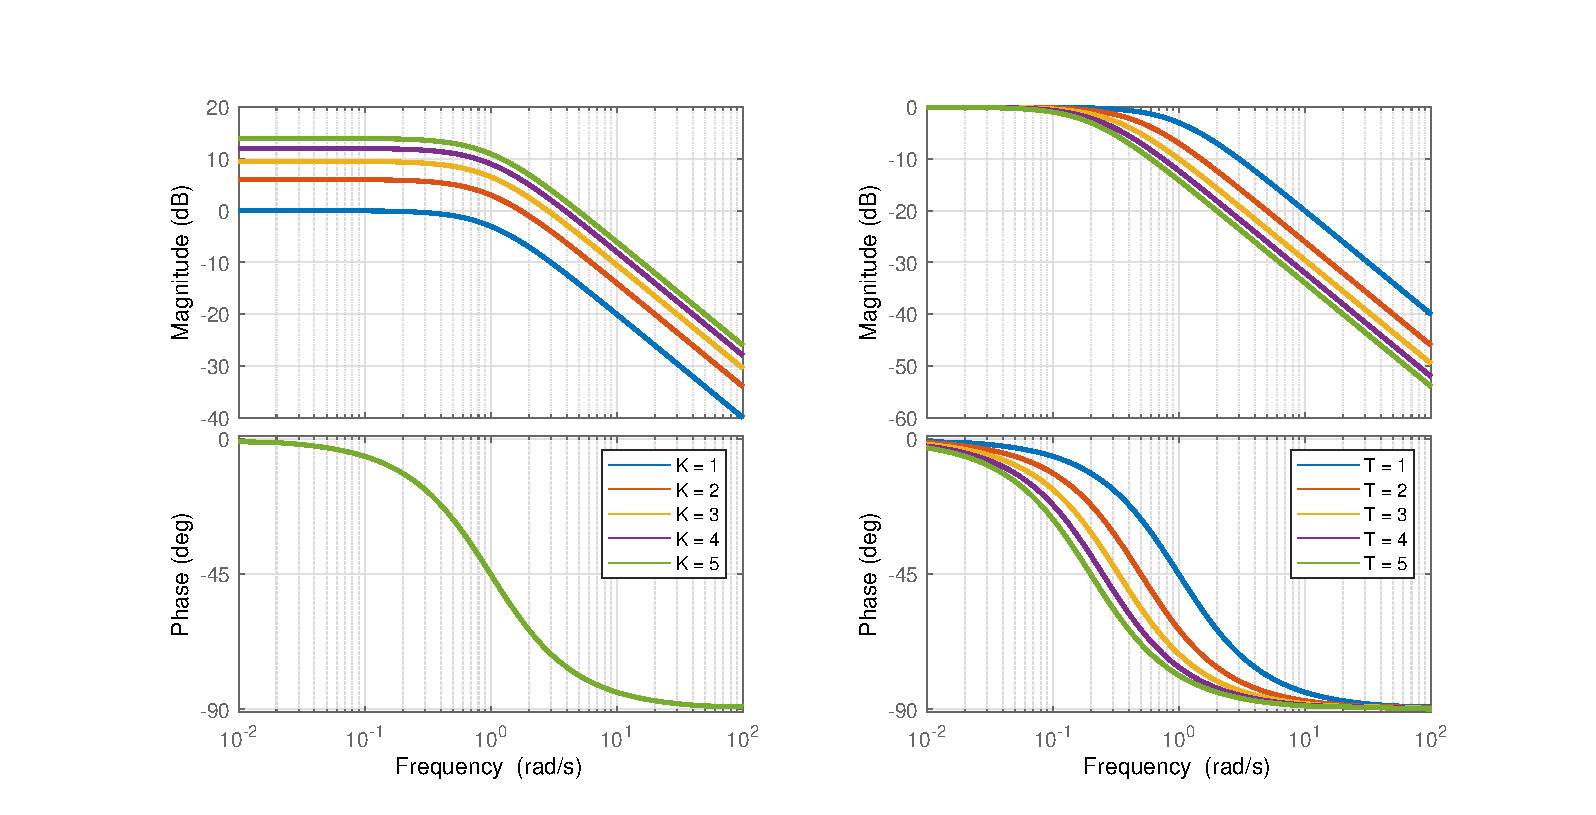
\includegraphics[width=1\textwidth]{images/bode3.eps}
        \caption{Bode plot for $G(s) = \frac{K}{Ts+1}$. \textbf{Left: $T=1$, $K\in [1,5]$. Right: $K=1$, $T\in [1,5]$.}}
    \end{figure}
\end{itemize}

\subsection{Bode Plots for 1\textsuperscript{st} Order Factor, $G(s) = (Ts+1)^{n}$}
\begin{itemize}
    \item \textbf{Gain plot}:
    \[
        20\log_{10}\lvert G(j\omega) \rvert
        = n\cdot 20\log_{10} \lvert Tj\omega+1 \rvert 
        = n\cdot20\log\sqrt{T^{2}\omega^{2}+1}\approx 
        \begin{cases}
            0                       & T \omega << 1\\
            n\cdot 20\log T\omega   & T \omega >> 0
        \end{cases}
    \]
    
    \item \textbf{Phase plot}:
    \[
        \angle G(j\omega) 
        = \angle (Tj\omega+1)^{n} 
        = n\cdot \tan^{-1}(T\omega) \approx 
        \begin{cases}
            0^{\circ}           & T\omega<<1\\
            n\cdot 45^{\circ}   & \omega=\omega_{c}=\frac{1}{T}\\
            n\cdot 90^{\circ}   & T\omega>>0\\
        \end{cases}
    \]
    
    \item Corner frequency $\omega_{c} = \frac{1}{T}$, \ slope = $n\cdot 20$ \textcolor{gray}{[dB/decade]}
\end{itemize}

\begin{figure}
    \centering
    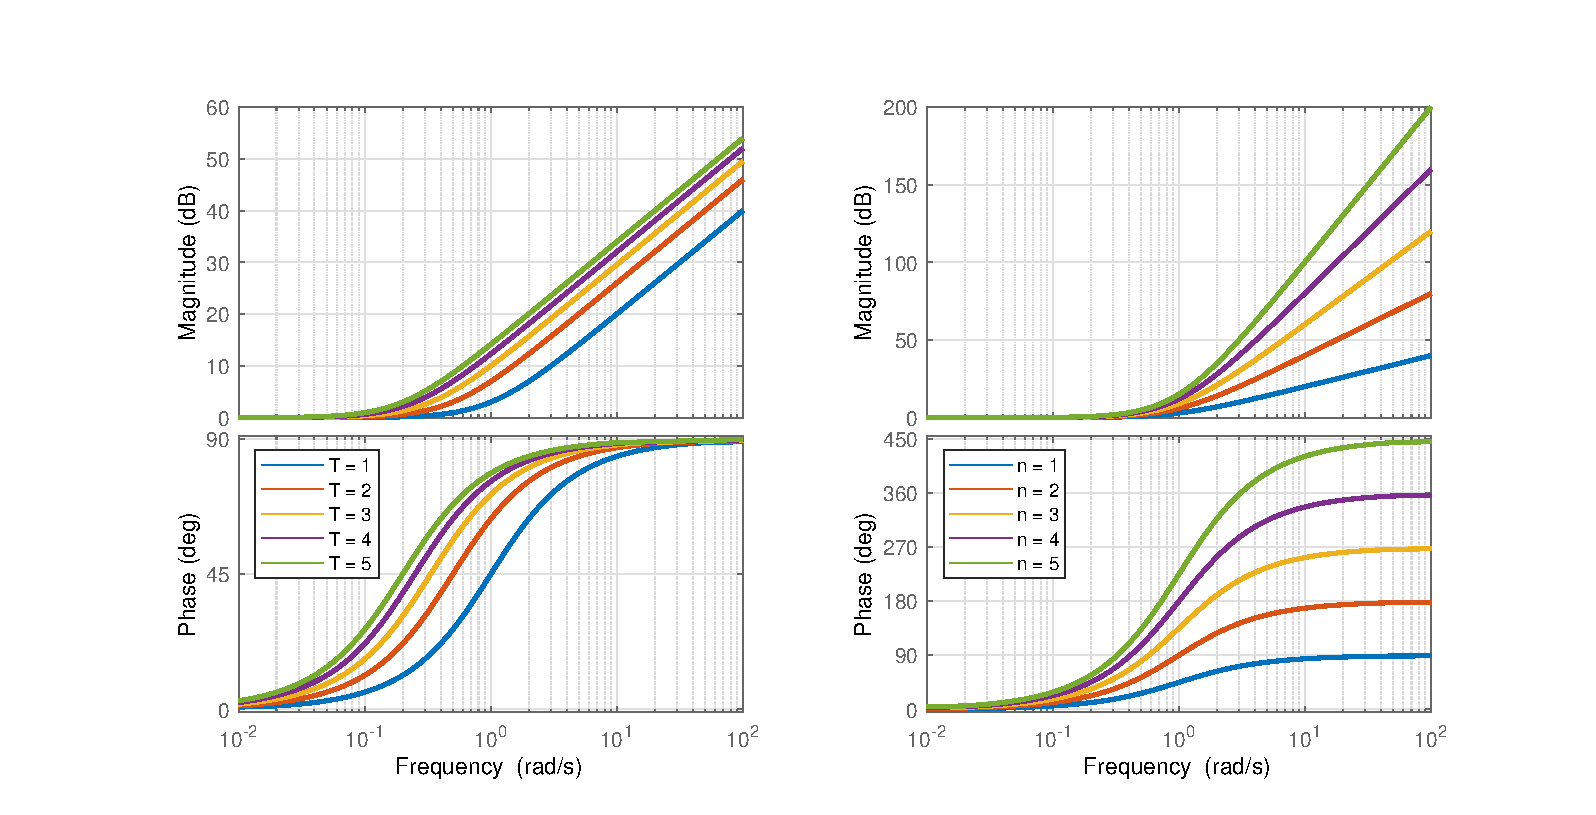
\includegraphics[width=\textwidth]{images/bode2.eps}
    \caption{Bode plot for $G(s) = (Ts+1)^{n}$. \textbf{Left: $n=1$, $T\in [1,5]$. Right: $T=1$, $n\in [1,5]$.}}
\end{figure}

\subsection{Bode Plots for 2\textsuperscript{nd} Order System, $G(s) = \frac{K\omega_{n}^{2}}{s^{2}+2\zeta\omega_{n}s+\omega_{n}^{2}}$}
Write the transfer function as a product of basic factors:
\[
    G(s) = \frac{K\omega_{n}^{2}}{s^{2}+2\zeta\omega_{n}s+\omega_{n}^{2}}=\frac{K}{-r^{2}+2\zeta jr +1}=\frac{K}{(1-r^{2})+2j\zeta r}
\]
where $r$ is known as the normalized frequency: $r = \frac{\omega}{\omega_{c}}$.

\begin{itemize}
    \item \textbf{Bode plot}:
    \[
        20\log_{10}\lvert G(j\omega) \rvert  =  20\log_{10} \bigg\lvert \frac{K}{(1-r^{2})+2j\zeta r} \bigg\rvert \approx 
        \begin{cases}
            20\log K            & r<<1 \\
            20\log K - 40\log r & r>>0
        \end{cases}
    \]

    \item \textbf{Phase plot}:
    \[
        \angle G(j\omega) = \angle \frac{K}{(1-r^{2})+2j\zeta r} =  \tan^{-1}(\frac{-2r\zeta}{1-r^{2}}) \approx 
        \begin{cases}
            0^{\circ}       & r<<1\\
            -90^{\circ}     & r = r_{c} = 1\\
            -180^{\circ}    & r>>0\\
        \end{cases}
    \]
    
    \item Resonant frequency $\omega_{r}$ at which the magnitude becomes max:
    \[
        \frac{d\lvert G(j\omega) \rvert}{dr}=0 \to r^{2} = q-2\zeta^{2}
    \]
    \[
        \omega_{r} = \omega_{n}\sqrt{1-2\zeta^{2}}
    \]
    Resonant peak magnitude at $\lvert G(j\omega_{r}) \rvert =\frac{1}{2\zeta\sqrt{1-\zeta^{2}}} $
\end{itemize}
%plots starts here!
\vspace{-.6cm}
\begin{figure}[H]
    \centering
    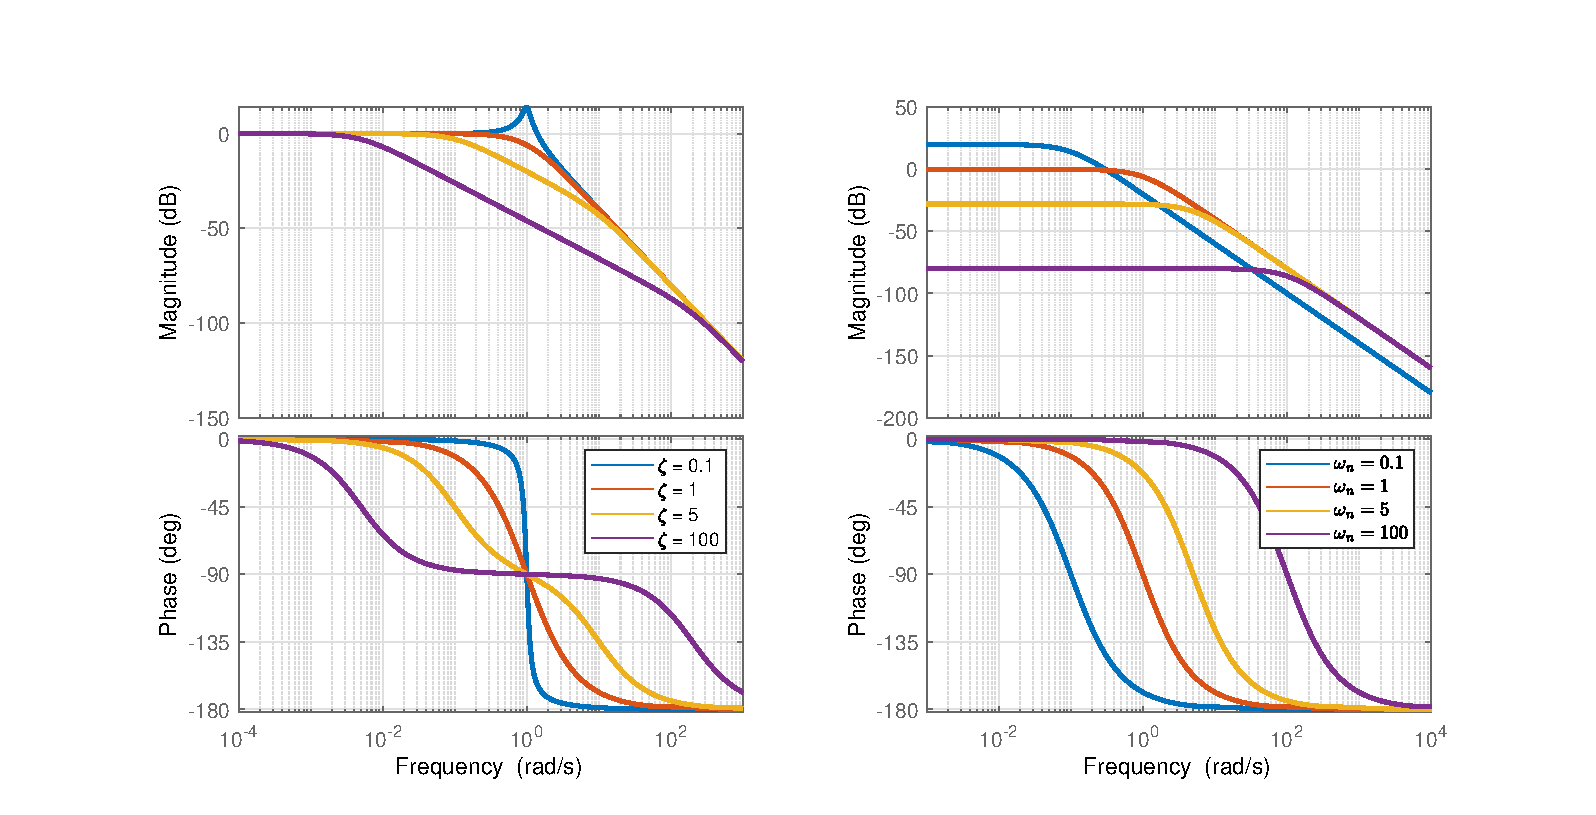
\includegraphics[width=\textwidth]{images/bode1.eps}
    \caption{Bode plot for $G(s) = \frac{K\omega_{n}^{2}}{s^{2}+2\zeta\omega_{n}s+\omega_{n}^{2}}$. \textbf{Left:} $\omega_{n}=1$, $\zeta$ varies. \textbf{Right:} $\zeta=1$, $\omega_{n}$ varies.}
\end{figure}

\subsection{Drawing Approximate Bode Plots}
\begin{enumerate}
\item Write the transfer function as a product of basic factors;
%---------------EXAMPLE START---------------%
    \begin{tcolorbox}[breakable, title=Example]
        \[G(s) = \frac{s+5}{(s+2)(s+4)}=\frac{5(0.2s+1)}{2(0.5s+1).4(0.25s+1)} = \frac{0.625. (0.2s+1)}{(0.5s+1)(0.25s+1)}\]
    \end{tcolorbox}
%----------------EXAMPLE END----------------%

    \item Identify the corner frequency for each factor;
%---------------EXAMPLE START---------------%
    \begin{tcolorbox}[breakable, title=Example cont'd]
        \[\omega_{c} = \frac{1}{0.5} , \frac{1}{0.25} , \frac{1}{0.2} = 2,4,5\]
    \end{tcolorbox}
%----------------EXAMPLE END----------------%

    \item Draw the \textbf{asymptotes between the corner frequencies} and \textbf{add the individual plots}.
        \begin{figure}[H] 
            \centering
            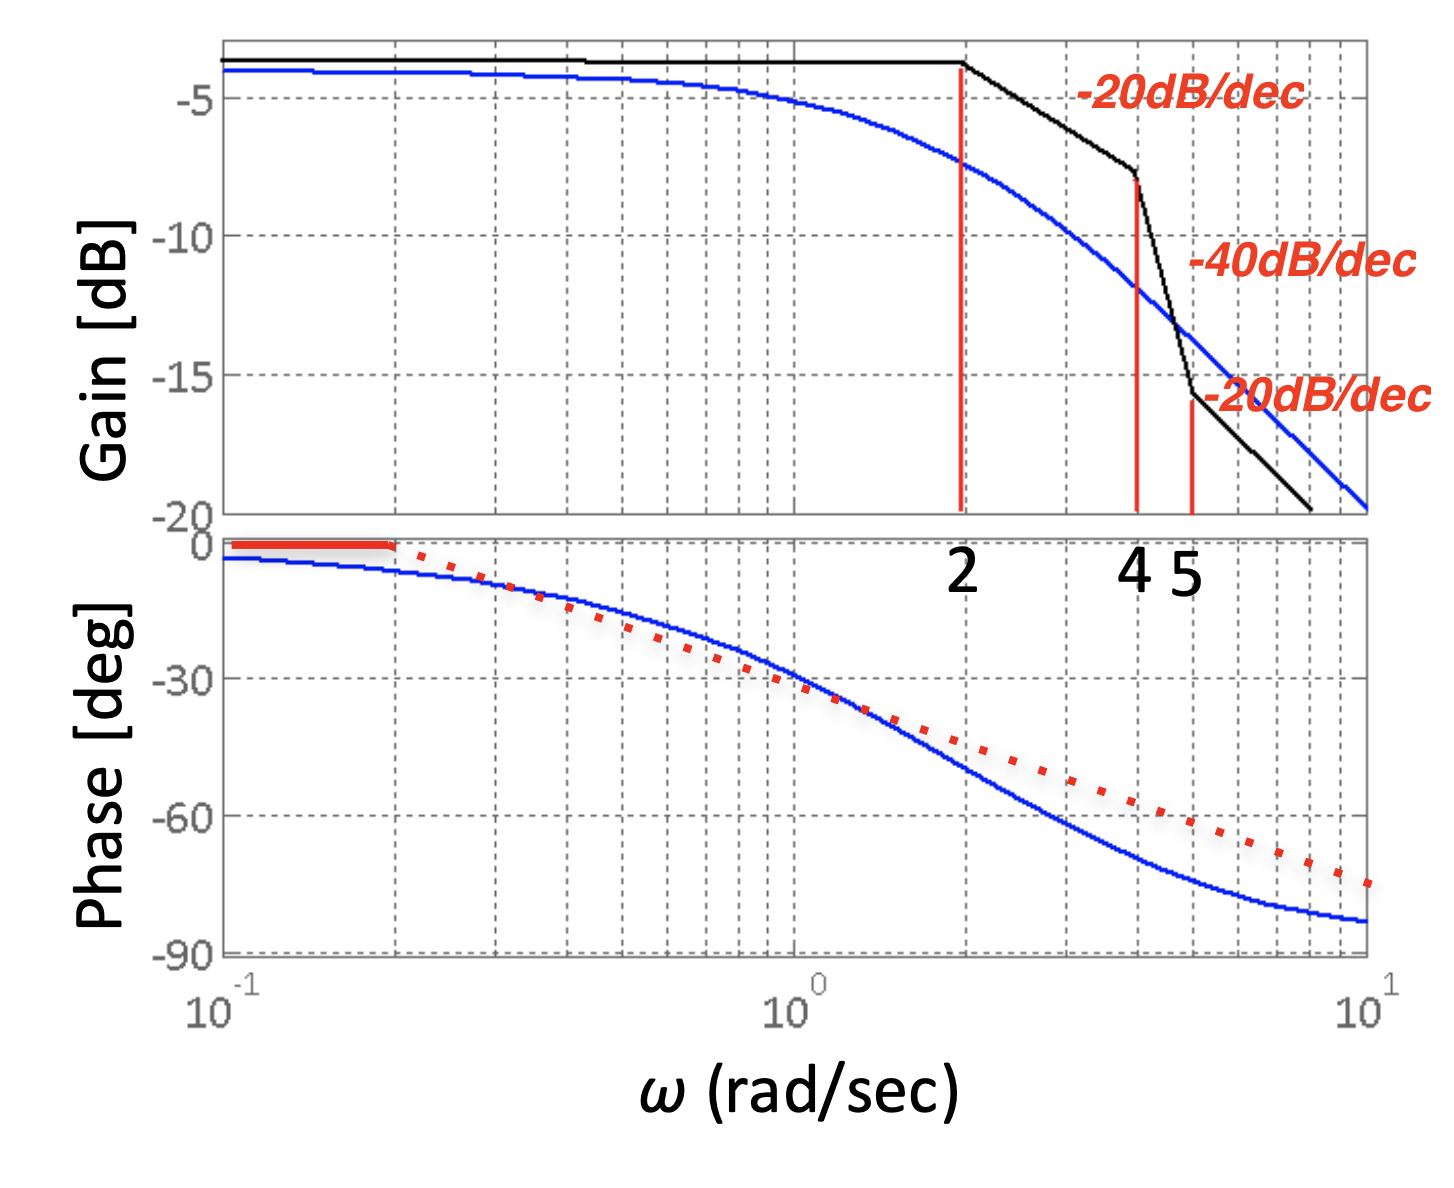
\includegraphics[width=.5\textwidth]{images/bode_plot.png}
        \end{figure}
\end{enumerate}

%-------------------------------------------%
\newpage
\section{Stability Margins}
%-------------------------------------------%
When designing a control system,  the first thing we want to ensure is the \textbf{stability} of the closed-loop system.

\begin{itemize}
    \item Stability margins measure how close the system is to instability: less margin, less stable
    
    \item There are 2 ways to make the system unstable:
    \begin{itemize}
        \item \textbf{Increase controller gain}, this reduces the \textbf{gain margin}.
        \item \textbf{Increase time delay}, this reduces the \textbf{phase margin}.
    \end{itemize}
    \begin{figure}[H] 
        \centering
        % 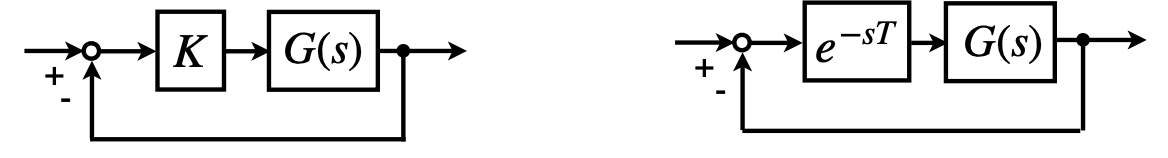
\includegraphics[width=0.75\textwidth]{images/unstable.png}
        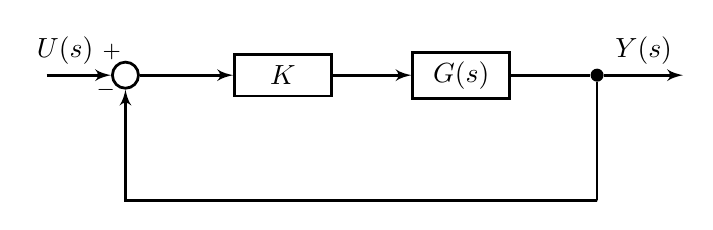
\begin{tikzpicture}[auto, node distance=2cm,>=latex',line width=1pt, scale=0.45]
    \node [input, name=input] {};
    \node [sum, right of=input] (sum) {};
    \node [block, right of=sum] (controller1) {$K$};
    \node [block, right= 1cm of controller1] (controller2) {$G(s)$};
    \coordinate [right=1cm of controller2, circle, scale=0.5, fill](tooutput){};
    \node [output, right=1cm of tooutput] (output) {};
    \coordinate [below= 1.5cm of tooutput] (measurements) {};

    \draw [draw,->] (input) -- node {$U(s)$\ {\footnotesize$+$}} (sum); 
    \draw [->] (sum) -- node {} (controller1);
    \draw [->] (controller1) -- (controller2);
    \draw [-] (controller2) -- (tooutput);
    \draw [->] (tooutput) -- node[] {$Y(s)$} (output);
    \draw [-] (tooutput) |- (measurements);
    \draw [->] (measurements) -| 
    node[pos=1] {{\footnotesize$-$}} (sum);
\end{tikzpicture}
\quad
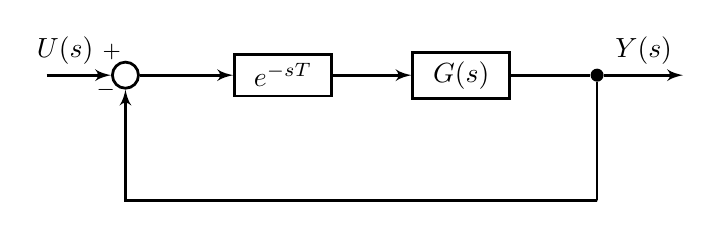
\begin{tikzpicture}[auto, node distance=2cm,>=latex',line width=1pt, scale=0.45]
    \node [input, name=input] {};
    \node [sum, right of=input] (sum) {};
    \node [block, right of=sum] (controller1) {$e^{-sT}$};
    \node [block, right= 1cm of controller1] (controller2) {$G(s)$};
    \coordinate [right=1cm of controller2, circle, scale=0.5, fill](tooutput){};
    \node [output, right=1cm of tooutput] (output) {};
    \coordinate [below= 1.5cm of tooutput] (measurements) {};

    \draw [draw,->] (input) -- node {$U(s)$\ {\footnotesize$+$}} (sum); 
    \draw [->] (sum) -- node {} (controller1);
    \draw [->] (controller1) -- (controller2);
    \draw [-] (controller2) -- (tooutput);
    \draw [->] (tooutput) -- node[] {$Y(s)$} (output);
    \draw [-] (tooutput) |- (measurements);
    \draw [->] (measurements) -| 
    node[pos=1] {{\footnotesize$-$}} (sum);
\end{tikzpicture}
        \caption{Two ways to make the system unstable}
    \end{figure}

    \item Two closed-loop, feedback systems have same characteristic functions. The open-loop transfer function, $C(s)H(s)$, determines the stability of the closed-loop systems:
    \begin{figure}[H] 
        \centering
        % 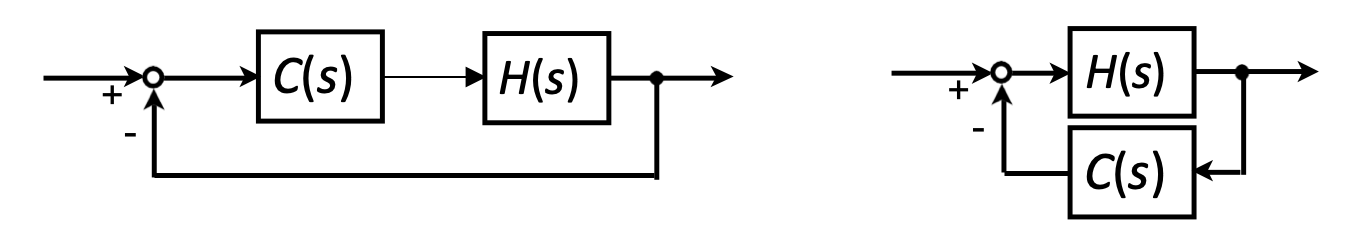
\includegraphics[width=0.65\textwidth]{images/closed_loop_stability.png}
        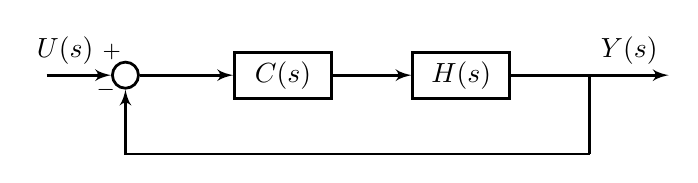
\begin{tikzpicture}[auto, node distance=2cm,>=latex',line width=1pt]
    \node [input, name=input] {};
    \node [sum, right of=input] (sum) {};
    \node [block, right of=sum] (controller1) {$C(s)$};
    \node [block, right= 1cm of controller1] (controller2) {$H(s)$};
    \coordinate [right=1cm of controller2](tooutput){};
    \node [output, right=1cm of tooutput] (output) {};
    \coordinate [below= 1cm of tooutput] (measurements) {};

    \draw [draw,->] (input) -- node {$U(s)$\ {\footnotesize$+$}} (sum); 
    \draw [->] (sum) -- node {} (controller1);
    \draw [->] (controller1) -- (controller2);
    \draw [-] (controller2) -- (tooutput);
    \draw [->] (tooutput) -- node[] {$Y(s)$} (output);
    \draw [-] (tooutput) |- (measurements);
    \draw [->] (measurements) -| 
    node[pos=1] {{\footnotesize$-$}} (sum);
\end{tikzpicture}

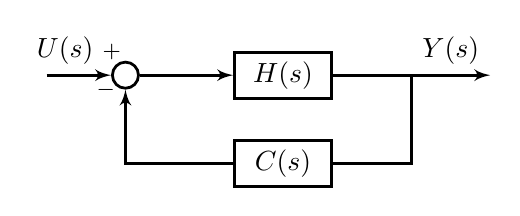
\begin{tikzpicture}[auto, node distance=2cm,>=latex',line width=1pt]
    \node [input, name=input] {};
    \node [sum, right of=input] (sum) {};
    \node [block, right of=sum] (controller1) {$H(s)$};
    \node [block, below= 0.5cm of controller1] (controller2) {$C(s)$};
    \coordinate [right=1cm of controller1](tooutput){};
    \node [output, right=1cm of tooutput] (output) {};

    \draw [draw,->] (input) -- node {$U(s)$\ {\footnotesize$+$}} (sum); 
    \draw [->] (sum) -- node {} (controller1);
    \draw [-] (controller1) -- (tooutput);
    \draw [-] (controller1) -- (tooutput) |- (controller2) ;
    \draw [->] (controller2) -| node[pos=1] {{\footnotesize$-$}} (sum);
    \draw [->] (tooutput) -- node[] {$Y(s)$} (output);
\end{tikzpicture}
    \end{figure} 
    
    \vspace{-1cm}
    \[
    G(s) = \frac{C(s)H(s)}{1+C(s)H(s)} \quad \quad \quad G(s) =\frac{H(s)}{1+C(s)H(s)} 
    \]\\
    The closed-loop system becomes unstable if the gain of the closed loop system is $\infty$. Specifically, in this case, denominator $\to 0$:
    \[
    1+C(s)H(s) =0 \quad \leftrightarrow  \quad \underbrace{C(s)H(s)}_{\text{open-loop transfer function}}=-1 \quad \leftrightarrow \quad \begin{cases}
    \lvert C(s)H(s) \rvert =1 \\
    \angle C(s)H(s) =-180^{\circ}\\
    \end{cases} 
    \]
    
    \item To make the Bode plot of $G_{D}(s) = C(s)H(s)$:
        \begin{figure}[H] 
            \centering
            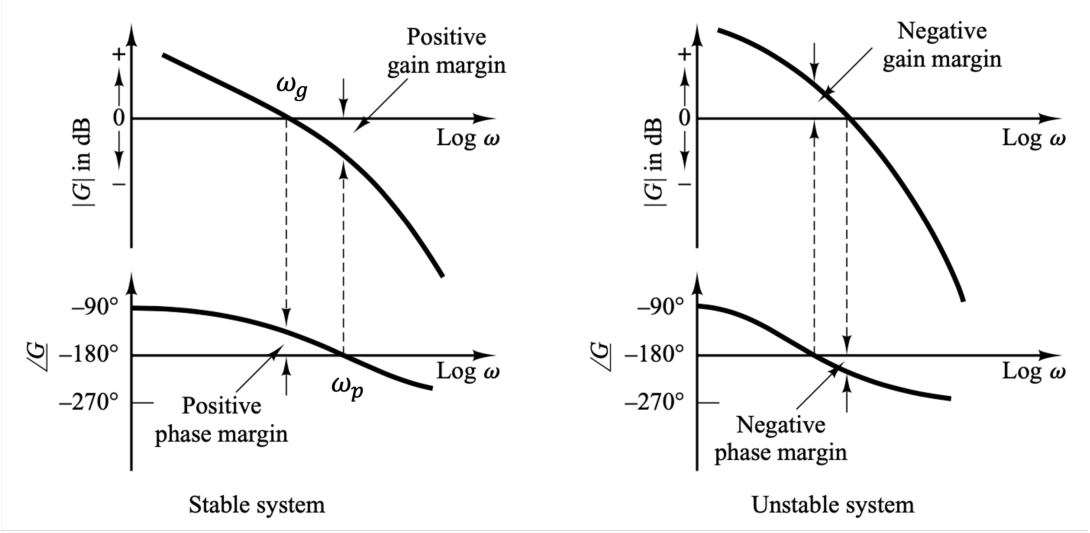
\includegraphics[width=0.85\textwidth]{images/margin.pdf}
            \caption{Stability margins for stable and unstable systems}
        \end{figure}
        
    \begin{itemize}
        \item Stability margin for stable systems: before losing the stability, we can 
        \begin{enumerate}
            \item add the same amount of \underline{phase delay} as the \textbf{positive phase margin}, at $\omega$, where $\lvert G(\omega)\rvert=0dB$
            \item add the same amount of \underline{gain} as the \textbf{positive phase margin}, at $\omega$, where $\angle G(\omega)=-180^{\circ}$
        \end{enumerate}
    
        \item Stability margin for unstable systems: the system can become stable if we 
            \begin{enumerate}
                \item reduce the same amount of \underline{phase delay} as the \textbf{negative phase margin}, at $\omega$, where $\lvert G(\omega)\rvert=0dB$
                \item reduce the same amount of \underline{gain} as the \textbf{negative gain margin}, at $\omega$, where $\angle G(\omega)=-180^{\circ}$
            \end{enumerate}
    \end{itemize}
\end{itemize}

%-------------------------------------------%
\subsection{Gain margin}
%-------------------------------------------%
The gain margin is the gain relative to $0dB$ when $\angle G(j\omega_{p}) = -180^{\circ}$:
 \[ GM = -20\log_{10}\lvert G(j\omega_{p})\rvert\]
 \ where $\omega_{p}$ is known as \textbf{phase cross-over frequency}, $\angle G(j\omega_{p}) = -180^{\circ}$. 

%-------------------------------------------%
\subsection{Phase margin}
%-------------------------------------------%
The \textbf{phase margin} is the phase relative to $180^{\circ}$ when $\lvert G(j\omega_{g}) \rvert =1$:
\[ PM = \angle G(j\omega_{g})-(-180^{\circ}) =\angle G(j\omega_{g})+ 180^{\circ}\] 
\ where $\omega_{g}$ is known as the \textbf{gain cross-over frequency}, $20\log \lvert G(j\omega_{g})\rvert = 0$.

%-------------------------------------------%
\subsection{Delay margin}
%-------------------------------------------%
Delay margin is the translation of phase margin in the delay time.
\[T = \frac{PM}{\omega_{g}}\frac{\pi}{180^{\circ}}\]
The system becomes unstable when the open-loop transfer function satisfies $e^{sT}G(s) = -1$ at the gain cross-over frequency, $\omega_{g}$.
\begin{align*}
\begin{split}
e^{-j\omega_{g}T}G(j\omega_{g})=-1
\quad \longrightarrow \quad 
 \angle (e^{j\omega_{g}T} G(j\omega_{g}))&= \angle (e^{j\omega_{g}T})+\angle G(j\omega_{g}) \\
&= -\omega_{g}T\cdot \frac{180^{\circ}}{\pi}+PM-180^{\circ} \\
&= -180^{\circ}
\end{split}
\end{align*}

%-------------------------------------------%
\newpage
\section{State-space Representation}
%-------------------------------------------%
\begin{itemize}
  \item \textbf{State-space representation} is a convenient way to describe \textbf{multi-input/multi-output} LTI systems in time domain using matrix algebra.
  
  \item The system is described as a set of inputs, $\mathbf{u}(t)$, outputs, $\mathbf{y}(t)$, and state variables, $\mathbf{x}(t)$.
  \begin{itemize}
    \item \textbf{State variables} is a set of variables that uniquely determines the current condition of the system (\textit{e.g.} position, temperature, protein concentration)
 \end{itemize}

    \begin{figure}[H] 
        \centering
        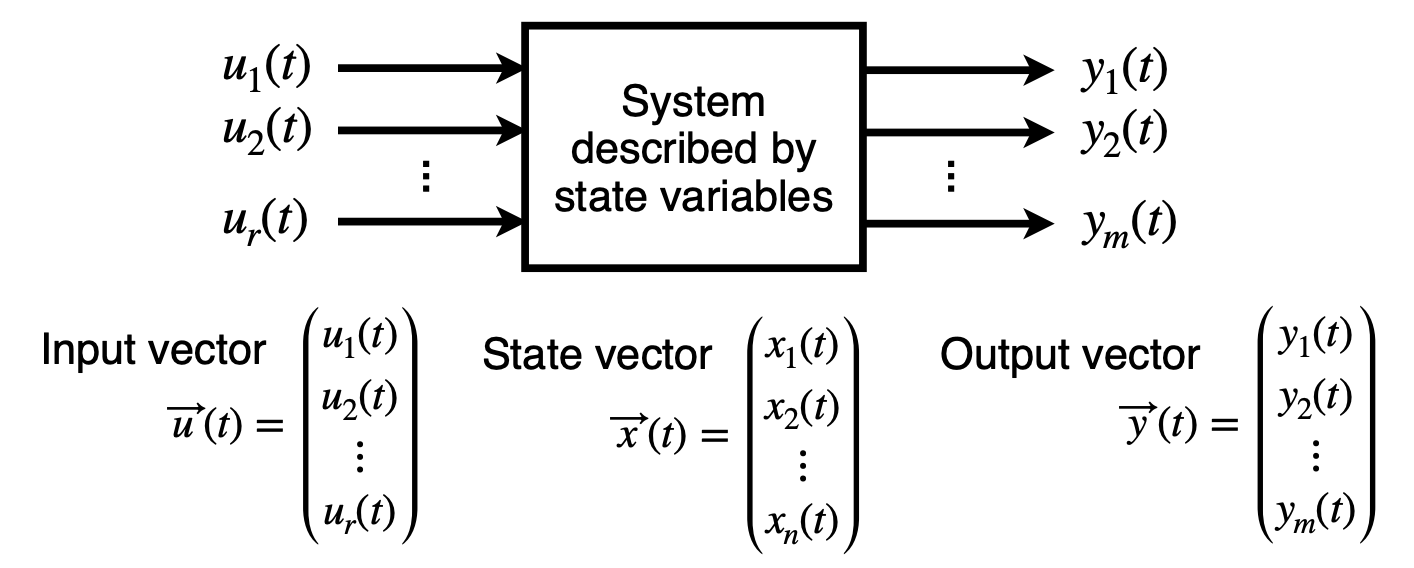
\includegraphics[width=0.65\textwidth]{images/multi_io.png}
        \caption{Multi-input/multi-output systems}
    \end{figure}

  \item The dynamics of state variables can be described by the 1$^{st}$ order differential equations, known as the \textbf{state equation}.
    \[\frac{d}{dt}\mathbf{x} = A\mathbf{x}+B\mathbf{u}\]
  \begin{itemize}
        \item $A$ is a $n\times n$ matrix, known as the \textbf{state matrix}, $ A \in \mathbb{R}^{n\times n}$.
        \item $B$ is a $n \times r$ matrix, known as the \textbf{input matrix}, $B \in \mathbb{R}^{n\times v}$.
  \end{itemize}
  
  \item \textbf{Output equation}: 
   \[\mathbf{y} = C\mathbf{x}+D\mathbf{u}\]
  \begin{itemize}
        \item $C$ is a $m\times n$ matrix, known as the \textbf{output matrix}, $ C \in \mathbb{R}^{m\times n}$.
        \item $D$ is a $m \times r$ matrix, known as the \textbf{feedthrough matrix}, $D \in \mathbb{R}^{m\times r}$.
  \end{itemize}
  
  \item \textbf{The transfer function} can be derived through taking the Laplace transform to the state-space model:
  \[G(s) = \frac{\mathbf{y}(s)}{\mathbf{u}(s)} = C(sI-A)^{-1}B+D\]
\end{itemize}
%---------------EXAMPLE START---------------%
\begin{ex}{}
\[G(s) = \frac{s+4}{s^{2}+3s+2} \quad \longleftrightarrow \quad (s^{2}+3s+2)Y(s) = (s+4)U(s)\]
This gives us a 2nd order O.D.E.
\[\ddot{y}+3\dot{y}+2y = \dot{u}+4u\]
\end{ex}
There are an infinite number of possible state-space models.
%----------------EXAMPLE END----------------%

%-------------------------------------------%
\subsection{Canonical Forms}
%-------------------------------------------%
Given a transfer function, there are infinite number of possible state-space representations.
\begin{itemize}
    \item A system is \textbf{controllable} if there exists an input that can move its state variable from an initial state to any arbitrary state in a finite time.
    
    \item A system is \textbf{observable} if its states at any time point can be determined by observing the output over a finite interval of time.
\end{itemize}

For the system:
\[ 
G(s) = \frac{Y(s)}{U(s)}=\frac{b_{1} s^{n-1}+b_{2} s^{n-2}+... +b_{n-1}s+b_{n}}{s^{n}+a_{1} s^{n-1}+...+a_{n-1}s+a_{n}} 
\]
\begin{itemize}
    \item The controllable canonical form is given by:
    \begin{gather*}
    \begin{pmatrix}
    \dot{x}_{1}\\
    \dot{x}_{2}\\
    \vdots\\
    \dot{x}_{n-1}\\
    \dot{x}_{n}
    \end{pmatrix} =
    \begin{pmatrix}
    0 & 1 & 0 & \ldots & 0\\
    0 & 0 & 1 & \ldots & 0 \\
    \vdots &\vdots &\vdots  & \ddots & \vdots \\
    0 & 0 & 0 & \ldots & 1\\
    -a_{n} & -a_{n-1} & -a_{n-2} & \ldots & -a_{1}
    \end{pmatrix} 
    \begin{pmatrix}
    {x}_{1}\\
    {x}_{2}\\
    \vdots\\
    {x}_{n-1}\\
    {x}_{n}
    \end{pmatrix}
    +
    \begin{pmatrix}
    0\\
    0\\
    \vdots\\
    0\\
    1
    \end{pmatrix}u
    \end{gather*}
    \begin{gather*}
    y = \begin{pmatrix}
    b_{n}&b_{n-1}&b_{n-1}&\ldots&b_{1}
    \end{pmatrix}
    \mathbf{x}
    \end{gather*}

%---------------EXAMPLE START---------------%
    \begin{ex}{}
    The system
    \[G(s) = \frac{s+4}{s^{2}+3s+2}\]
    can be written as (in controllable canonical form)
    \begin{gather*}
    \begin{pmatrix}
    \dot{x}_{1}\\
    \dot{x}_{2}\\
    \end{pmatrix} = 
    \begin{pmatrix}
    0&1\\
    -2&-3\\
    \end{pmatrix}
    \begin{pmatrix}
    x_{1}\\
    x_{2}\\
    \end{pmatrix}
    +
    \begin{pmatrix}
    0\\
    1\\
    \end{pmatrix}u
    \end{gather*}
    \begin{gather*}
    y = 
    \begin{pmatrix}
    4&1\\
    \end{pmatrix}
    \begin{pmatrix}
    x_{1}\\
    x_{2}\\
    \end{pmatrix}
    +0u
    \end{gather*}
    To verify this, start from the definition of the transfer function:
    \begin{equation*}
    \begin{aligned}
    G(s) &= \frac{\mathbf{y}(s)}{\mathbf{u}(s)} = C(sI-A)^{-1}B+D\\
    &= \begin{pmatrix}
     4 & 1\\
    \end{pmatrix}
    \{sI-\begin{pmatrix}
    0&1\\
    -2&-3\\
    \end{pmatrix}
    \}^{-1}
    \begin{pmatrix}
    0\\
    1\\
    \end{pmatrix}\\
    &=\begin{pmatrix}
     4 & 1\\
    \end{pmatrix}
    \begin{pmatrix}
    s&-1\\
    2&s+3\\
    \end{pmatrix}
    ^{-1}
    \begin{pmatrix}
    0\\
    1\\
    \end{pmatrix}\\
    &=\begin{pmatrix}
     4 & 1\\
    \end{pmatrix}
    \frac{1}{s(s+3)+2}
    \begin{pmatrix}
    s+3&1\\
    -2&s\\
    \end{pmatrix}
    \begin{pmatrix}
    0\\
    1\\
    \end{pmatrix}\\
    &= \frac{s+4}{s(s+3)+2}
    \end{aligned}
    \end{equation*}
    \end{ex}
%----------------EXAMPLE END---------------%


    \item The observable canonical form is given by:
    \begin{gather*}
    \begin{pmatrix}
    \dot{x}_{1}\\
    \dot{x}_{2}\\
    \vdots\\
    \dot{x}_{n-1}\\
    \dot{x}_{n}
    \end{pmatrix} =
    \begin{pmatrix}
    0 & 0 &  \ldots & 0& -a_{n}\\
    1 & 0 &  \ddots &  \vdots &  -a_{n-1}\\
    0 &1 &\ddots  & \vdots & \vdots \\
    \vdots & \ddots & \ddots & 0 & -a_{2}\\
    0 & \ldots & 0 & 1 & -a_{1}
    \end{pmatrix} 
    \begin{pmatrix}
    {x}_{1}\\
    {x}_{2}\\
    \vdots\\
    {x}_{n-1}\\
    {x}_{n}
    \end{pmatrix}
    +
    \begin{pmatrix}
    b_{n}\\
    b_{n-1}\\
    \vdots\\
    b_{2}\\
    b_{1}
    \end{pmatrix}u
    \end{gather*}
    \begin{gather*}
    y = \begin{pmatrix}
    0&0&\ldots&0&1\\
    \end{pmatrix}
    \mathbf{x}
    \end{gather*}

%---------------EXAMPLE START---------------%
    \begin{ex}{}
        The system 
        \[G(s) = \frac{s+4}{s^{2}+3s+2}\]
        can be written as  (in observable canonical form)
        \begin{gather*}
        \begin{pmatrix}
        \dot{x}_{1}\\
        \dot{x}_{2}\\
        \end{pmatrix} = 
        \begin{pmatrix}
        0&-2\\
        1&-3\\
        \end{pmatrix}
        \begin{pmatrix}
        x_{1}\\
        x_{2}\\
        \end{pmatrix}
        +
        \begin{pmatrix}
        4\\
        1\\
        \end{pmatrix}u
        \end{gather*}
        \begin{gather*}
        y = 
        \begin{pmatrix}
        0&1\\
        \end{pmatrix}
        \begin{pmatrix}
        x_{1}\\
        x_{2}\\
        \end{pmatrix}
        +0u
        \end{gather*}
        To verify this, start from the definition of the transfer function:
        \begin{equation*}
        \begin{aligned}
        G(s) &= \frac{\mathbf{y}(s)}{\mathbf{u}(s)} = C(sI-A)^{-1}B+D\\
        &= \begin{pmatrix}
         0 & 1\\
        \end{pmatrix}
        \{sI-\begin{pmatrix}
        0&-2\\
        1&-3\\
        \end{pmatrix}
        \}^{-1}
        \begin{pmatrix}
        4\\
        1\\
        \end{pmatrix}\\
        &=\begin{pmatrix}
         0 & 1\\
        \end{pmatrix}
        \begin{pmatrix}
        s&2\\
        -1&s+3\\
        \end{pmatrix}
        ^{-1}
        \begin{pmatrix}
        4\\
        1\\
        \end{pmatrix}\\
        &=\begin{pmatrix}
         0 & 1\\
        \end{pmatrix}
        \frac{1}{s(s+3)+2}
        \begin{pmatrix}
        s+3&-2\\
        1&s\\
        \end{pmatrix}
        \begin{pmatrix}
        4\\
        1\\
        \end{pmatrix}\\
        &= \frac{s+4}{s(s+3)+2}
        \end{aligned}
        \end{equation*}
    \end{ex}
%----------------EXAMPLE END----------------%
\end{itemize}


%-------------------------------------------%
\subsection{Stability of State-space Model}
%-------------------------------------------%
The system is stable if all eigenvalues of $A$ satisfies $\Re(\lambda_{i})<0$. \textit{i.e.} All eigenvalues of $A$ are on the left-side of the s-plane.\\\\
There are 2 ways to find the matrix exponential:
\begin{itemize}
    \item Diagonalisation of $A$;
    \item Using the identity: $e^{At} = \mathcal{L}^{-1}(sI-A)^{-1}$.
\end{itemize}


%-------------------------------------------%
\subsubsection{Solutions of State-space Model}
%-------------------------------------------%
\[\mathbf{x}(t) = \underbrace{e^{At}\mathbf{x}(0)}_{\text{zero-input response}}+\underbrace{\int_{0}^{t}e^{A(t-\tau)}B\mathbf{u}(\tau)d\tau}_{\text{zero-state response}}\]
\[\mathbf{y}(t) = Ce^{At}\mathbf{x}(0)+C\int_{0}^{t}e^{A(t-\tau)}B\mathbf{u}(\tau)d\tau+D\mathbf{u}(\tau)\]

%---------------EXAMPLE START---------------%
\begin{ex}{}
Find the response of the system where 
\begin{gather*}
\mathbf{\dot{x}}=\begin{pmatrix} -
2&0\\
1&-1
\end{pmatrix}
\mathbf{x}+
\begin{pmatrix}
1\\0
\end{pmatrix}u
\end{gather*}
and $\mathbf{x}(0)=\begin{pmatrix} 0\\0 \end{pmatrix}$, $u(t)=5$, $y =\begin{pmatrix}
2&1\\
\end{pmatrix}
 \mathbf{x}$
\vspace{.2cm}\hrule
\[\mathbf{x}(t) = e^{At}\mathbf{x}(0)+\int_{0}^{t}e^{A(t-\tau)}B\mathbf{u}(\tau)d\tau\]
Since\footnote{derivation see below}
\[e^{At} = \begin{pmatrix}
e^{-2t} & 0\\
e^{-t}-e^{-2t} & e^{-t}\\
\end{pmatrix}
\]
Therefore
\begin{equation*}
\begin{aligned}
\mathbf{x}(t) &= \begin{pmatrix}
e^{-2t} & 0\\
e^{-t}-e^{-2t} & e^{-t}\\
\end{pmatrix}
\int^{t}_{0}
\begin{pmatrix}
e^{-2\tau} & 0\\
e^{-\tau}-e^{2\tau} & e^{-\tau}
\end{pmatrix}
\begin{pmatrix}
5\\
0\\
\end{pmatrix}d\tau\\\\
&=\begin{pmatrix}
e^{-2t} & 0\\
e^{-t}-e^{-2t} & e^{-t}\\
\end{pmatrix}
\begin{pmatrix}
\int_{0}^{t} 5e^{2\tau}d\tau\\
\int_{0}^{t} (5e^{\tau}-5e^{2\tau})d\tau\\
\end{pmatrix}\\\\
&=\begin{pmatrix}
\frac{5}{2}(1-e^{-2t})\\
\frac{5}{2}(1+e^{-2t})-5e^{-t}
\end{pmatrix}
\end{aligned}
\end{equation*}

\begin{gather*}
y = (2 \ 1)\mathbf{x} = (2 \ 1)\begin{pmatrix}
\frac{5}{2}(1-e^{-2t})\\
\frac{5}{2}(1+e^{-2t})-5e^{-t}
\end{pmatrix}
 = \frac{15}{2}-\frac{5}{2}e^{-2t}-5e^{-t}
\end{gather*}

\vspace{.3cm}\hrule\vspace{.3cm}
Matrix exponential: $e^{tA} = Ve^{tD}V^{-1}$
\[tA = V(tD)V^{-1}\]
When eigenvalues of $A$ are $\lambda_{1}$, $\lambda_{2}$, ...Eigenvalues of $tA$ are $t\lambda_{1}$, $t\lambda_{2}$, ...
\[e^{tA} = \sum^{\infty}_{k=0}\frac{(tA)^{k}}{k!} =\sum^{\infty}_{k=0}\frac{V(tA)^{k}V^{-1}}{k!} = V\bigg(\sum^{\infty}_{k=0}\frac{(tA)^{k}}{k!}\bigg)V^{-1} \]

\begin{equation*}
\begin{aligned}
\sum^{\infty}_{k=0}\frac{(tA)^{k}}{k!}  &=\sum^{\infty}_{k=0}\frac{1}{k!} \begin{pmatrix}
(t\lambda_{1})^{k}&0&\ldots&0\\
0&(t\lambda_{2})^{k}&\ldots&0\\
\vdots&\vdots&\ddots&\vdots\\
0&0&\ldots&(t\lambda_{n})^{k}
\end{pmatrix}\\\\
&=\begin{pmatrix}
\sum^{\infty}_{k=0}\frac{(t\lambda_{1})^{k}}{k!} &0&\ldots&0\\
0& \sum^{\infty}_{k=0}\frac{(t\lambda_{2})^{k}}{k!}&\ldots&0\\
\vdots&\vdots&\ddots&\vdots\\
0&0&\ldots&\sum^{\infty}_{k=0}\frac{(t\lambda_{n})^{k}}{k!}
\end{pmatrix}\\\\
&=\begin{pmatrix}
e^{t\lambda_{1}}&0&\ldots&0\\
0&e^{t\lambda_{2}}&\ldots&0\\
\vdots&\vdots&\ddots&\vdots\\
0&0&\ldots&e^{t\lambda_{n}}
\end{pmatrix}\\\\
&= e^{tD}
\end{aligned}
\end{equation*}
\end{ex}
%----------------EXAMPLE END----------------%


%-------------------------------------------%
\subsubsection{Impulse Response}
%-------------------------------------------%
Transfer function\[G(s) = \frac{\mathbf{y}(s)}{\mathbf{u}(s)}=C(sI-A)^{-1}B+D\]
Impulse response\[\mathbf{y}(t) = Ce^{At}B+D\]
\begin{equation*}
\begin{split}
    \frac{d}{dt}e^{At} = Ae^{At} \xrightarrow{\mathcal{L}} & s\mathcal{L}(e^{At})-e^{A0} = A\mathcal{L}(e^{At})\\
    &(sI-A)\mathcal{L}(e^{At}) = e^{A0} = I\\
    &\mathcal{L}(e^{At}) = (sI-A)^{-1}\\
    &e^{At} = \mathcal{L}^{-1}(sI-A)^{-1}\\
\end{split}
\end{equation*}

%-------------------------------------------%
\subsubsection{Stability of State-space Models}
%-------------------------------------------%
\begin{align*}
\begin{split}
    G(s) &= C(sI-A)^{-1}B+D \\
    &=C\frac{1}{det(sI-A)}(sI-A)^{T}_{cofactor}B+D
\end{split}
\end{align*}
Poles $s$ of $G(s)$ = Eigenvalues $\lambda$ of $A$.
\[det(sI-A) = det(\lambda I-A) = 0\]
System is stable \textit{if and only if} $\Re (\lambda_{i})<0$ for all eigenvalues $\lambda_{i}$ of $A$.
 
 
%-------------------------------------------%
\subsubsection{Pole Placement}
%-------------------------------------------%
\begin{itemize}
\item \textbf{SISO system}: Poles of the closed-loop system as a function of the gain $K$: $\displaystyle \frac{Y(s)}{R(s)} = \frac{G(s)}{1+KG(s)}$.
\begin{figure}[H] 
    \centering
    % 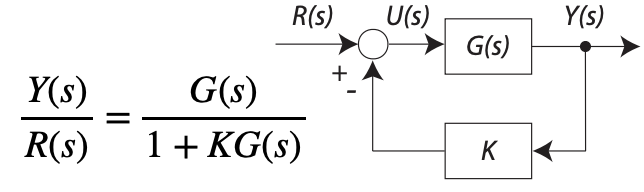
\includegraphics[width=0.4\textwidth]{images/SISO.png}
    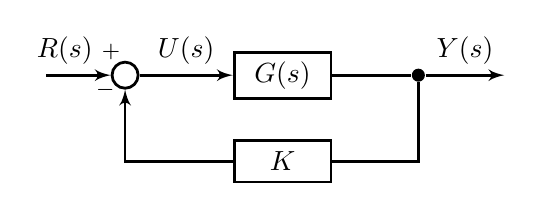
\begin{tikzpicture}[auto, node distance=2cm,>=latex', line width = 1pt]
    \node [input, name=input] {};
    \node [sum, right of=input] (sum) {};
    \node [block, right of=sum] (controller1) {$G(s)$};
    \node [block, below= 0.5cm of controller1] (controller2) {$K$};
    \coordinate [right=1cm of controller1, circle, scale=0.5, fill](tooutput){};
    \node [output, right=1cm of tooutput] (output) {};

    \draw [draw,->] (input) -- node {$R(s)$\ {\footnotesize$+$}} (sum); 
    \draw [->] (sum) -- node {$U(s)$} (controller1);
    \draw [-] (controller1) -- (tooutput);
    \draw [-] (controller1) -- (tooutput) |- (controller2) ;
    \draw [->] (controller2) -| node[pos=1] {{\footnotesize$-$}} (sum);
    \draw [->] (tooutput) -- node[] {$Y(s)$} (output);
\end{tikzpicture}
    \caption{SISO system}
\end{figure}
\item \textbf{MIMO system}: 
\[\dot{x} = Ax+Bu = Ax +B(r-Kx) = (A-BK)x+Br\]
Eigenvalues of the matrix $(A-BK)$ determines the closed-loop stability.

\begin{figure}[H] 
    \centering
    % 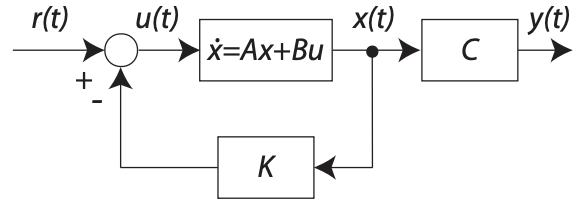
\includegraphics[width=0.4\textwidth]{images/MIMO.png}
    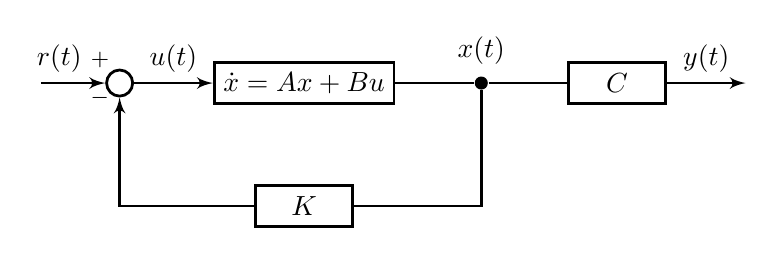
\begin{tikzpicture}[auto, node distance=2cm,>=latex', line width=1pt]
    \node [input, name=input] {};
    \node [sum, right of=input] (sum) {};
    \node [block, right= 1cm of sum] (controller1) {$\dot{x}=Ax+Bu$};
    \node [block, below= 1cm of controller1] (controller2) {$K$};
    \node [right=1cm of controller1, circle, fill, scale=0.5](tocon3){};
    \node [block, right= 1cm of tocon3] (controller3) {$C$};
    \node [output, right=1cm of controller3] (output) {};

    \draw [draw,->] (input) -- node {$r(t)$\ {\footnotesize$+$}} (sum); 
    \draw [->] (sum) -- node {$u(t)$} (controller1);
    \draw [-] (controller1) -- (tocon3)node[above = .1cm]{$x(t)$};
    \draw [->] (tocon3) -- node {} (controller3) -- node[]{$y(t)$}(output);
    
    \draw [->](tocon3) |- (controller2) -| node[pos=1] {{\footnotesize$-$}} (sum);
\end{tikzpicture}
    \caption{MIMO system}
\end{figure}
\end{itemize}
%---------------EXAMPLE START---------------%
\begin{ex}{}
\begin{equation*}
\begin{pmatrix}
\dot{x}_{1}\\
\dot{x}_{2}\\
\end{pmatrix} = 
\begin{pmatrix}
-0.5&-0.8\\
0.8&0\\
\end{pmatrix}
\begin{pmatrix}
x_{1}\\
x_{2}\\
\end{pmatrix}
+\begin{pmatrix}
1\\
0\\
\end{pmatrix}
u
\end{equation*}
Poles at $-0.25\pm 0.76\mathbf{j}$.\ \\
Design a state-feedback:
\begin{equation*}
\hat{u} = \begin{pmatrix}
k_{1} & k_{2}\\
\end{pmatrix}
\begin{pmatrix}
x_{1}\\
x_{2}\\
\end{pmatrix}
\end{equation*}
So that the closed-loop system has the poles at $-1$ and $-2$:
\begin{equation*}
A-BK = \begin{pmatrix}
-0.5&-0.8\\
0.8&0\\
\end{pmatrix}-
\begin{pmatrix}
1\\
0\\
\end{pmatrix}
\begin{pmatrix} 
k_{1}&k_{2}\\
\end{pmatrix}
 = 
 \begin{pmatrix}
 -0.5-k_{1}&-0.8-k_{2}\\
 0.8&0\\
 \end{pmatrix}
\end{equation*}
\begin{equation*}
det\{\lambda I-(A-BK)\} = \begin{vmatrix}
\lambda+0.5+k_{1} & 0.8+k_{2}\\
-0.8&\lambda\\
\end{vmatrix}
= (\lambda +1)(\lambda +2) 
\end{equation*}
\[ \lambda(\lambda + 0.5 + k_{1}) + 0.8(0.8 + k_{2}) = (\lambda +1)(\lambda +2) \]
This gives two solutions: $k_{1}=2.5$ and $k_{2}=1.7$
\end{ex}
%----------------EXAMPLE END----------------%


%-------------------------------------------%
\subsection{Decouple Interconnected Systems}
%-------------------------------------------%
\subsubsection{Relationship Between Equivalent Systems}
The system \[G(s)=\frac{1}{(s-1)(s-2)}\] can be written in
controllable canonical form:
\begin{gather*}
\begin{pmatrix}
\dot{x}_{1}\\
\dot{x}_{2}\\
\end{pmatrix}
= \underbrace{\begin{pmatrix}
0 & 1\\
-2 &3 \\
\end{pmatrix}}_{A_{1}}
\begin{pmatrix}
x_{1}\\
x_{2}\\
\end{pmatrix}
+\begin{pmatrix}
0\\
1\\
\end{pmatrix} u
\end{gather*}
and observable canonical form:
\begin{gather*}
\begin{pmatrix}
\dot{x}_{1}\\
\dot{x}_{2}\\
\end{pmatrix}
= \underbrace{\begin{pmatrix}
0 & -2\\
1 &3 \\
\end{pmatrix}}_{A_{2}}
\begin{pmatrix}
x_{1}\\
x_{2}\\
\end{pmatrix}
+\begin{pmatrix}
1\\
0\\
\end{pmatrix}
u
\end{gather*}
Since the two forms come from one transfer function, the system stability must be the same.
More importantly, $A$ matrix determine the stability of the system.\\\\
Relationship between $A_{1}$ and $A_{2}$:
\begin{gather*}
\begin{pmatrix}
-5 & 1\\
1 & 1 \\
\end{pmatrix}
\begin{pmatrix}
0 & 1\\
-2 &3 \\
\end{pmatrix}
=
\begin{pmatrix}
0 & -2\\
1 &3 \\
\end{pmatrix}
\begin{pmatrix}
-5 & 1\\
1 & 1 \\
\end{pmatrix}
\end{gather*}
\[TA_{1} = A_{2}T \quad \leftrightarrow \quad A_{1}=T^{-1}A_{2}T\]
Moreover,  both matrices $A_{1}$, $A_{2}$ has same eigenvalues at 1 and 2. So $A_{1}$, $A_{2}$ can be digonalized to the same matrix.
\[D = \begin{pmatrix}
1 & 0\\
0 & 2\\
\end{pmatrix}
\]
with the relation
\[A_{1}V_{1} = V_{1}D \quad \quad A_{2}V_{2} = V_{2}D\]

\subsubsection{Decoupling of Interconnected Systems (\textit{from Math 2})}
Decoupling of interconnected systems are done by matrix digonalization. 
\begin{figure}[H] \centering
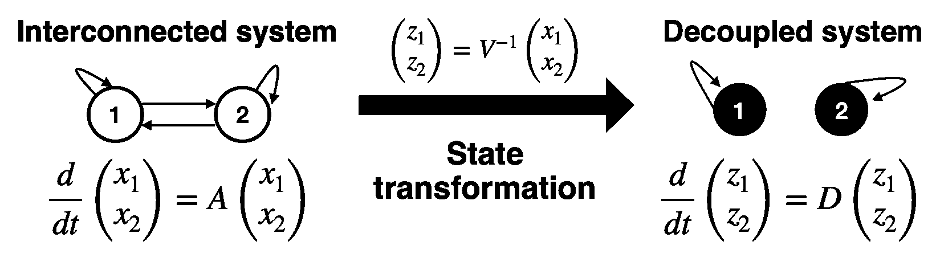
\includegraphics[width=.8\textwidth]{images/decouple.png}
\caption{De-couple an interconnected system}
\end{figure} \ \\
Decoupling of the interconnected system allows us to analyze the dynamics of a large system by only considering smaller systems.

%---------------EXAMPLE START---------------%
\begin{ex}{}
\begin{itemize}
\item Interconnected system:
\begin{equation*}
\frac{d}{dt} 
\begin{pmatrix}
x_{1}\\
x_{2}\\
\end{pmatrix}
=A
\begin{pmatrix}
x_{1}\\
x_{2}\\
\end{pmatrix}\quad \xrightarrow{A_{1}=\begin{pmatrix}
0 & 1\\
-2 & 3\\
\end{pmatrix}} \quad 
\begin{pmatrix}
\dot{x}_{1}\\
\dot{x}_{2}\\
\end{pmatrix} = 
\begin{pmatrix}
0 & 1\\
-2 & 3\\
\end{pmatrix}
\begin{pmatrix}
x_{1}\\
x_{2}\\
\end{pmatrix} = \begin{pmatrix}
x_{2}\\
-2x_{1}+3x_{2}\\
\end{pmatrix}
\end{equation*}

$\dot{x}_{1}$ and $\dot{x}_{2}$ depend on $x_{1}$ and $x_{2}$, this means the system is interconnected. 
\item Decoupled system:
\begin{equation*}
\frac{d}{dt} 
\begin{pmatrix}
z_{1}\\
z_{2}\\
\end{pmatrix}
=D
\begin{pmatrix}
z_{1}\\
z_{2}\\
\end{pmatrix} \quad \xrightarrow{D=\begin{pmatrix}
1 & 0\\
0 & 2\\
\end{pmatrix}} \quad 
\begin{pmatrix}
\dot{z}_{1}\\
\dot{z}_{2}\\
\end{pmatrix} = 
\begin{pmatrix}
1 & 0\\
0 & 2\\
\end{pmatrix}
\begin{pmatrix}
z_{1}\\
z_{2}\\
\end{pmatrix} = \begin{pmatrix}
z_{1}\\
2z_{2}\\
\end{pmatrix}
\end{equation*}
$\dot{z}_{1}$ only depends on $z_{1}$ and $\dot{z}_{2}$ only depends on $z_{2}$, this means the system is decoupled. 
\item The matrix D can be obtained by digonalization of matrix A
\[D =  V^{-1}AV\]
 \ where $V$ is the eigenvector.
\item The relationship between $z_{1}$, $z_{2}$ and $x_{1}$, $x_{2}$ satisfies:
\begin{gather*}
\begin{pmatrix}
z_{1}\\
z_{2}\\
\end{pmatrix}
=V^{-1}
\begin{pmatrix}
x_{1}\\
x_{2}\\
\end{pmatrix}
\end{gather*}
In this case:
\[V = \begin{pmatrix}
2&-1\\
-1&2\\
\end{pmatrix}\]
Therefore:
\begin{gather*}
\begin{pmatrix}
z_{1}\\
z_{2}\\
\end{pmatrix}
= 
\begin{pmatrix}
2&-1\\
-1&1\\
\end{pmatrix}
\begin{pmatrix}
x_{1}\\
x_{2}\\
\end{pmatrix}
\end{gather*}
\end{itemize}
\end{ex}
%----------------EXAMPLE END----------------%

%-------------------------------------------%
\subsection{Controllability and Observabiliy}
%-------------------------------------------%
\subsubsection{Controllability}
\begin{itemize}
    \item A system is controllable if there exists an input that can move its state variable from an initial state to any arbitrary state in a finite time;
    
    \item A systems is controllable if the controllability matrix is of full rank
    \[rank (B \ AB\ A^{2}B \ ...\ A^{n-1}B)=n\]
\end{itemize}

\subsubsection{Observability}
\begin{itemize}
    \item A system is observable if its states at any time point can be determined by observing the output over a finite interval of time.
    
    \item A system is observable if the observability matrix is of full rank.
\end{itemize}

\[rank \begin{pmatrix}
C       \\
CA      \\
CA^{2}  \\
\vdots  \\
CA^{n-1}
\end{pmatrix} 
= n
\]

\subsubsection{Stabilisability and Detectability}
\begin{itemize}
    \item A system is stabilisable if all the uncontrollable states are stable.
    
    \item A systems is detectable if all the unobservable states are stable.
\end{itemize}


\end{document}